
% !TeX spellcheck = pt_BR
% !TEX encoding = UTF-8 Unicode

\chapter{Funções}\label{Cap:Funcoes}

\ifdefined\updateans
% Only need to run once in a lifetime, when the file ans.tex needs to be updated.
\Writetofile{ans}{\protect\section*{Capítulo \ref{Cap:Funcoes}}}
\fi

O conceito de \emph{função}\index{função} será o principal assunto 
tratado neste curso.
Neste capítulo daremos algumas definições elementares, e consideraremos
algumas das funções mais usadas na prática, que são as funções 
trigonométricas e as
potências (exponenciais e logaritmos serão estudadas no próximo capítulo).
Também começaremos a falar de \emph{gráfico de uma função} desde a Seção
\ref{Sec:Graficos}.\\

A noção de função aparece quando uma grandeza depende de 
uma outra. Por exemplo:

\begin{itemize}
\item Uma partícula evolui na reta. A \emph{trajetória} é uma função que 
dá a sua posição em função do tempo:
$$t\mapsto x(t)\,.$$

\item 
O \emph{volume} e a \emph{superfície} de uma esfera são duas funções que 
dependem ambas do raio:
$$r\mapsto \tfrac{4}{3}\pi r^3\,,\quad r\mapsto 4\pi r^2\,.$$

\item 
Um gás está contido num recipiente hermeticamente fechado, de 
temperatura fixa mas de volume variável. A \emph{pressão} no recipiente 
é função do volume:
$$v\mapsto p(v)\,.$$
\end{itemize}

\section{Definição e exemplos}

Como visto acima, uma \grasA{função} $f$ (de uma variável real) é um 
mecanismo que, a um número real 
$x$, chamado \grasA{entrada} (ou \grasA{variável}), associa um
único número real construído a partir de 
$x$, denotado $f(x)$ e chamado \grasA{saída} (ou \grasA{imagem}). Essa associação costuma
ser denotada: 
$$x\mapsto f(x)\,.$$
Neste curso, a entrada e a saída serão ambos números reais.
Veremos em breve que cada função precisa ser definida com um \emph{domínio}.

\begin{ex}
 A função ``multiplicação por dois'' $x\mapsto 2x$ (por exemplo $3\mapsto 6$, $-13\mapsto
-26$),
 a função ``valor absoluto'' $x\mapsto |x|$ (por exemplo $3\mapsto 3$, $-13 \mapsto 13$),
a função ``quadrado'' $x\mapsto x^2$ (por exemplo $3\mapsto 9$, $-13\mapsto 169$), e a
função ``valor inteiro'' $x\mapsto \lfloor x\rfloor$, onde $\lfloor x\rfloor$ é o maior
número inteiro menor ou igual a $x$ (por exemplo $3\mapsto 3$, $1.5\mapsto 1$,
$-3.1415\mapsto -4$), são todas bem definidas para qualquer real $x\in \bR$.
\end{ex}

\begin{ex}\label{Ex:Umsobrex}
%\emph{Excluir a divisão por zero.}
Para definir a função ``inverso'', $x\mapsto \frac{1}{x}$, é
preciso evitar uma divisão por zero, isto é, somente tomar uma entrada $x\in \bR\setminus
\{0\}$. 
Assim, a função $f(x)=\tfrac{1}{x}$ é bem definida uma vez que escrita da seguinte maneira:
\begin{align*}
 f:\bR\setminus \{0\}&\to \bR\\
x&\mapsto \tfrac{1}{x}\,.
\end{align*}
Do mesmo jeito, para definir $f(x)=\tfrac{x}{x^2-1}$, é preciso excluir os valores em que
o denominador é zero\index{divisão por zero}:
\begin{align*}
 f:\,\bR\setminus\{-1,+1\}&\to \bR\\
x&\mapsto \tfrac{x}{x^2-1}\,.
\end{align*}
\end{ex}

Os dois últimos exemplos mostram que em geral, uma função deve ser definida {junto} com o
seu \grasA{domínio}\index{domínio}, que dá os valores de $x$ para os quais $f(x)$ é
definida. O domínio será em geral denotado por $D$:
\begin{align*}
f:\,D&\to \bR\\
x&\mapsto f(x)\,.
\end{align*}
O domínio será importante para garantir que $f(x)$ seja bem definida. Mas às
vezes, poderemos escolher um domínio particular somente por razões específicas, ou pelas
exigências de um problema.

\begin{ex}
 As funções trigonométricas encontradas no Capítulo \ref{Cap_Fundam} podem ser
consideradas como \emph{funções} no sentido acima. 
O seno, por exemplo, associa ao ângulo $\alpha$ de um triângulo retângulo a razão do lado
oposto sobre a hipotenusa: $\alpha\mapsto\sen \alpha$.\index{seno! função}
Aqui vemos que, pela origem geométrica do problema, é necessário especificar os valores
possíveis 
de $\alpha$: para o triângulo ser bem definido, o ângulo precisa tomar valores entre $0$ e 
 $\tfrac{\pi}{2}$ (de fato, é delicado falar de ``lado oposto'' para um ângulo nulo ou
maior que 
$\tfrac{\pi}{2}$). 
 Para indicar que a função assim definida pega a sua entrada no intervalo
$(0,\tfrac{\pi}{2})$, escreveremos
\begin{align*}
 \sen:(0,\tfrac{\pi}{2})&\to \bR\\
\alpha&\mapsto \sen \alpha\,.
\end{align*}

% \begin{center}
% \begin{bmlimage}\begin{tikzpicture}[scale=1]
% \pgfmathsetmacro{\a}{2.3};
% %\draw (-\a,0) -- (0,0);
% % \draw[thick, gray] (0,0) grid[step=0.5] (6,3); 
% % \draw[very thin, gray] (0,0) grid[step=0.1] (6,3);
% \draw[ ->] (0,0) -- (0,\a);
% \draw[ ->] (0,0)-- (\a,0);
% \draw [color=\coulseno, thick] (1.1,1.665)--(1.1,0) node[midway, above, sloped]{$\sen \alpha$};
% \draw[dotted] (2,0) arc (0:90:2);
% \draw(0,0)--(1.1,1.665);
% \draw (0.5,1.1) node{$1$};
% \draw[ ->] (0.5,0) arc (0:1 r:0.5);
% \draw (0.4,0.3) node[right]{$\alpha$};
% \fill (1.1,1.665) circle (0.45mm);
% \pgfmathsetmacro{\h}{8};
% \draw (3-\h,1) node[right]{$\sen:(0,\tfrac{\pi}{2})\to \bR$};
% \draw (4.65-\h,0.5) node[right]{$\alpha\mapsto \sen \alpha$};
% \end{tikzpicture}\end{bmlimage}
% \end{center}

No entanto vimos que, usando o círculo trigonométrico\index{círculo trigonométrico}, o
seno
de qualquer ângulo (mesmo negativo) pode ser definido, o que permite estender ele à reta
real inteira:
\begin{align*}
 \sen:\bR&\to \bR\\
\alpha&\mapsto {\sen \alpha}\,.
\end{align*}
A função cosseno\index{cosseno! função} se define de maneira análoga. Mas, com a
tangente, uma restrição é necessária. 
 De fato, $\tan \alpha=\frac{\sen \alpha}{\cos \alpha}$ e, a divisão por zero sendo
proibida, a tangente não é definida para ângulos $\alpha\in \bR$ tais que $\cos\alpha=0$.
Logo (veja o Exercício \ref{exoequacoestrigo}), 
\begin{align*}
 \tan:\bR\setminus\{\pisobredois k\pi,k\in\bZ\}&\to \bR\\
\alpha&\mapsto {\tan \alpha}\,.
\end{align*}
\end{ex}

\begin{ex}
\emph{A função raiz.}\index{raiz! função} Seja $a\in \bR$, e considere a equação
\eq{\label{eqparadefraiz}z^2=a\,.}
 Sabemos (ver Seção \ref{SecEquacoes}) que se $a<0$, essa equação não possui soluções, se
$a=0$ ela possui a única solução $z=0$, e se $a> 0$, ela possui duas soluções:
$z=+\sqrt{a}$ e $z=-\sqrt{a}$. Nesses dois últimos casos, quando $a\geq 0$, definiremos 
a \grasA{função raiz de $a$} como sendo a solução positiva de \eqref{eqparadefraiz}, isto
é, $+\sqrt{a}$.
 Quando $a<0$, a função raiz de $a$ não é definida. Assim, a função raiz $x\mapsto
f(x)=\sqrt{x}$
é bem definida somente quando $x\geq 0$, o que se escreve da seguinte maneira:
\begin{align*}
 f:\,\bR_+&\to \bR\\
x&\mapsto \sqrt{x}\,.
\end{align*}
\end{ex}

Por exemplo, para achar o domínio da função $\sqrt{1-x}$, é necessário que $1-x\geq 0$, 
isto é, que $x\leq 1$. Logo,
\begin{align*}
 f:\,(-\infty,1]&\to \bR\\
x&\mapsto \sqrt{1-x}\,.
\end{align*}

\begin{exo}
Determine os domínios das seguintes funções:
\begin{multicols}{4}
\begin{enumerate}
\item\label{itte1} $\frac{1}{x^2+3x-40}$
\item\label{itte2} $\frac{x}{x}$
\item\label{itte21} $|x-1|$
\item\label{itte3} $\frac{x+1}{x^2+1}$
\item\label{itte4} $\frac{1}{1-\frac{1-x}{x}}$
\item\label{itte45} $\sqrt{x-1}$
\item\label{itte46} $\sqrt{x^2-1}$
\item\label{itte5} $\frac{1}{1-\sqrt{x-1}}$
\item\label{itdominio1} $\frac{8x}{1-x^2}$
\item\label{itdominio2} $\frac{8x}{\sqrt{1-x^2}}$
\item\label{itdominio3} $\sqrt{2x-1-x^2}$
\item\label{itdominio4} $\frac{\sqrt{2x-x^2}}{\sqrt{2-x-x^2}}$
\item\label{itdominio41} $\frac{1}{\cos x}$
\item\label{itdominio5} $\sqrt{{\sen x}}$
\item\label{itdominio6} $\sqrt{x}-\sqrt{x}$
\item\label{itdominio7} $\sqrt{1-\sqrt{1+x^2}}$
\end{enumerate}
\end{multicols}
\vspace{0.01cm}
\begin{sol}
\eqref{itte1} $D=\bR\setminus\{-8,5\}$ 
\eqref{itte2} $D=\bR\setminus\{0\}$ 
\eqref{itte21} $D=\bR$
\eqref{itte3} $D=\bR$ 
\eqref{itte4} $D=\bR\setminus\{0,\tfrac12\}$ 
\eqref{itte45} $D=[1,\infty)$
\eqref{itte46} $D=(-\infty,-1]\cup [1,\infty)$ 
\eqref{itte5} $D=[1,\infty ) \setminus \{2\}$
\eqref{itdominio1} $D=\bR\setminus\{\pm 1\}$
\eqref{itdominio2} $D=(-1,+1)$
\eqref{itdominio3} $D=\{1\}$
 \eqref{itdominio4} $D=[0,1)$ (Atenção: é necessário que o numerador \emph{e} o
denominador sejam bem definidos.)
\eqref{itdominio41} $D=\bR\setminus \{\pisobredois+k\pi, k\in \bZ\}$ 
\eqref{itdominio5} $D=$união dos intervalos $[k2\pi,\pi +k2\pi]$, para $k\in \bZ$.
 \eqref{itdominio6} $D=\bR_+$. Observe que apesar da função ser identicamente nula, o seu
domínio não é a reta toda.
\eqref{itdominio7} $D=\{0\}$ (e não $D=\varnothing$!).
\end{sol}
\end{exo}

\subsection{Limitação}\index{função! limitada}
Vimos que a função $f(x)=\tfrac{1}{x}$ é bem definida quando $x\neq 0$, mas observemos
agora o que acontece com $f(x)$ para os valores de $x$ perto de $0$. Por exemplo, para os
valores de $x$ positivos $x=0.1$, $x=0.01$, ...
$$
 \tfrac{1}{0.1}=10\,,\quad \tfrac{1}{0.01}=100\,,\quad
\tfrac{1}{0.001}=1000\,,\quad\dots\quad\,,\,\tfrac{1}{0.0000001}=10000000\,\dots.
$$
Assim, vemos que a medida que $x>0$ se aproxima de zero, $\tfrac{1}{x}$ atinge valores
positivos arbitrariamente grandes. O mesmo fenômeno acontece para os valores de $x<0$:
$\tfrac{1}{x}$ atinge valores negativos arbitrariamente grandes.
Diz-se que a função é \emph{não-limitada}.\\

Uma função $f$ com domínio $D$ é dita \grasA{limitada superiormente} se existir um 
número finito $M_+$
tal que
$$f(x)\leq M_+\quad \forall x\in D\,.$$
Por outro lado, $f$ é dita \grasA{limitada inferiormente} se existir um número
finito $M_-$ tal que
$$f(x)\geq M_-\quad \forall x\in D\,.$$
Se $f$ for limitada inferiormente \emph{e} superiormente, então ela é
\grasA{limitada}.\\

\begin{ex}
A função seno é limitada. De fato, pela definição (olhe para o círculo trigonométrico),
$-1\leq \sen x\leq 1$. Aqui podemos tomar $M_+=1$, $M_-=-1$.
\end{ex}

\begin{ex} Como visto acima, a função $\tfrac{1}{x}$ não é limitada, nem
inferiormente nem superiormente. 
Por outro lado, $\tfrac{1}{x^2}$ não é limitada superiormente, pois
pode tomar valores arbitrariamente grandes a medida que $x$ se aproxima de zero.
No entanto, como $\tfrac{1}{x^2}\geq 0$, ela é limitada inferiormente
(podemos escolher $M_-=0$, ou $M_-=-3$, ou qualquer outro número negativo).

Do mesmo jeito, a função $f(x)=\frac{x}{x^2-1}$ (Exemplo
\ref{Ex:Umsobrex}) é não-limitada, pois toma valores arbitrariamente grandes
(negativos ou positivos) quando $x$ se aproxima de $+1$ ou $-1$.
\end{ex}

\begin{ex}
 Considere $f(x)=\frac{x^2}{x^2+1}$. Observe que $f$ é sempre não-negativa, e que o
numerador é menor do que o denominador para qualquer $x$: $x^2\leq x^2+1$. Logo,
$$0\leq f(x)=\frac{x^2}{x^2+1}\leq \frac{x^2+1}{x^2+1}=1\,,$$
o que prova que $f$ é limitada (por exemplo com $M_-=0$, $M_+=1$).
\end{ex}

\begin{exo}
Determine quais das funções abaixo são limitadas.
\begin{multicols}{3}
\begin{enumerate}
\item\label{itlimitacao1} $x^2$
 \item\label{itlimitacao2} $\tan x$
\item\label{itlimitacao3} $\frac{1}{x^2+1}$
\item\label{itlimitacao4} $\frac{1}{\sqrt{1-x}}$
\item\label{itlimitacao5} $\frac{x-1}{x^3-x^2+x-1}$
\item\label{itlimitacao6} $x+\sen x$
\end{enumerate}
\end{multicols}
\vspace{0.01cm}
\begin{sol}
\eqref{itlimitacao1} $x^2$ é limitada inferiormente ($M_-=0$) mas não
superiormente: toma valores arbitrariamente grandes quando
$x$ toma valores grandes. \eqref{itlimitacao2} Não-limitada. De fato, $\tan x=\frac{\sen
x}{\cos x}$, e quando $x$ se aproxima por exemplo de $\pisobredois$, $\sen x$ se aproxima
de $1$ e $\cos x$ de $0$, o que dá uma divisão por zero. (Dê uma olhada no gráfico da
função tangente mais longe no capítulo.) \eqref{itlimitacao3} É limitada: 
$\tfrac{1}{x^2+1}\geq 0\equiv M_-$, e como $x^2+1\geq
1$, temos 
$\frac{1}{x^2+1}\leq \tfrac11=1\equiv M_+$. \eqref{itlimitacao4} Limitada
inferiormente ($M_-=0$), mas não superiormente: o domínio
dessa função é $(-\infty,1)$, e quando $x<1$ se aproxima de $1$, $\sqrt{1-x}$ se aproxima
de zero, o que implica que $\frac{1}{\sqrt{1-x}}$ toma valores arbitrariamente grandes.
\eqref{itlimitacao5} Observe que o denominador $x^3-x^2+x-1$ se anula em $x=1$. Logo, o
domínio da função é $\bR\setminus \{1\}$. Fatorando (ou fazendo a divisão),
$x^3-x^2+x-1=(x-1)(x^2+1)$. Portanto, quando $x\neq 1$,
$\frac{x-1}{x^3-x^2+x-1}=\frac{x-1}{(x-1)(x^2+1)}=\frac{1}{x^2+1}$. Como $\frac{1}{x^2+1}$
é limitada (item \eqref{itlimitacao3}), $\frac{x-1}{x^3-x^2+x-1}$ é limitada.
\eqref{itlimitacao6} Não-limitada. Apesar de $\sen x$ ser limitado por $-1$ e $+1$, 
o ``$x$'' pode tomar valores arbitrariamente grandes.
\end{sol}
\end{exo}

\section{Gráfico}\label{Sec:Graficos}\index{gráfico}
Um dos nossos objetivos é de entender, pelo menos de maneira
qualitativa, a dependência de uma função $f(x)$ em relação à sua
variável $x$. Uma jeito de
proceder é representar a função no plano cartesiano, via o seu
\emph{gráfico}. O gráfico permite extrair 
a informação essencial contida na função, de maneira intuitiva, pois
\emph{geométrica}.\\

Seja $f$ uma função com domínio $D$. 
\grasA{Esboçar o gráfico de $f$} consiste em traçar todos os pontos do plano cartesiano
da forma $(x,f(x))$, 
onde $x\in D$. Por exemplo, se $f$ tem um domínio $D=[a,b]$, 
\begin{center}
\begin{bmlimage}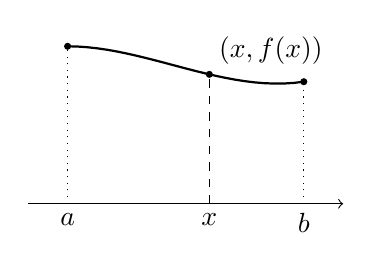
\begin{tikzpicture}
\coordinate (A) at (0,0);
\coordinate (B) at (3,0);
\pgfmathsetmacro{\x}{1.8}
\coordinate (X) at (\x,0);
\draw [->] (-0.5,0)--(3.5,0);
\draw (A) node{$\shortmid$};
%\fill (A) circle (0.35mm);
\draw (A) node[below]{$a$};
%\draw[thick] (A)--(B);
\draw (B) node{$\shortmid$};
%\fill (B) circle (0.35mm);
\draw (B) node[below]{$b$};
\draw (X) node{$\shortmid$};
\draw (X) node[below]{$x$};
\draw[dashed] (X)--(\x,{0.05*\x^3-0.2*(\x)^2+2}) node[above right]{$(x,f(x))$};
\draw [thick, domain=0:3] plot (\x,{0.05*\x^3-0.2*(\x)^2+2});
\fill (\x,{0.05*\x^3-0.2*(\x)^2+2}) circle (0.45mm);
\draw[dotted] (A)--(0,2);
\draw[dotted] (B)--(3,{0.05*3^3-0.2*3^2+2});
\fill (0,2) circle (0.45mm);
\fill (3,{0.05*3^3-0.2*3^2+2}) circle (0.45mm);
\end{tikzpicture}\end{bmlimage}
\end{center}
Ao $x$ percorrer o seu domínio $[a,b]$, o ponto $(x,f(x))$ traça o gráfico de $f$.

\begin{ex}\label{Ex:retaegrafico}\index{reta}
\emph{Retas não-verticais} são gráficos de um tipo particular. Por exemplo, 
se $f(x)=\tfrac{x}{2}+1$ é considerada com o domínio $D=[0,2)$, o seu gráfico 
é um pedaço da reta de inclinação\index{inclinação} $\tfrac12$ com
ordenada na origem igual a $1$: 
\begin{center}
\begin{bmlimage}\begin{tikzpicture}
\draw [ ->] (0,-0.1)--(0,2) node[left]{$y$};
\draw [ ->] (-0.3,0)--(2.5,0) node[right]{$x$};
\draw [thick] (0,1)--(2,2);
\draw (0,0) node{$\shortmid$};
\fill[intfechado] (0,1) circle (0.55mm);
\fill[intaberto] (2,2) circle (0.55mm);
\pgfmathsetmacro{\x}{0.8};
\draw (\x,0) node{$\shortmid$};
\draw (\x,0) node[below]{$x$};
\draw[dashed] (\x,0)--(\x,{1+\x/2});
\fill (\x,{1+\x/2}) circle (0.45mm);
\draw (0,0) node[below]{$0$};
\draw (2,0) node[below]{$2$};
\draw[dotted] (2,0)--(2,2);
\draw [decorate, decoration=brace] (-0.05,0)--(-0.05,1) node[midway, left]{$1$};
\end{tikzpicture}\end{bmlimage}
\end{center}
Observe que uma reta vertical \emph{não define o gráfico de uma
função}.
\end{ex}

\begin{ex}
Façamos o esboço da função $f(x)=|x|$, com domínio $D=[-1,2]$. Lembre
que pela definição de valor absoluto em \eqref{eq:defvalorabs},
$|x|=x$ se $x\geq 0$, e $|x|=-x$ se $x<0$.
Portanto, o gráfico de $f$ é: 1) entre $-1$ e $0$, a reta de
inclinação $-1$ passando pela origem, 2) entre $0$ e $2$, a reta de
inclinação $1$ passando pela origem:
\begin{center}
\begin{bmlimage}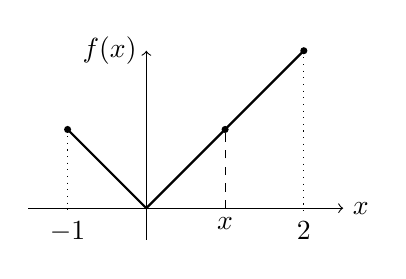
\begin{tikzpicture}
\draw [ ->] (-1.5,0)--(2.5,0) node[right]{$x$};
\draw [ ->] (0,-0.4)--(0,2) node[left]{$f(x)$};
\draw[thick] (-1,1)--(0,0)--(2,2);
\draw[dotted] (-1,1)--(-1,-0.05) node[below]{$-1$};
\draw[dotted] (2,2)--(2,-0.05) node[below]{$2$};
%%%%%%%
\pgfmathsetmacro{\x}{1};
\pgfmathsetmacro{\y}{abs(\x)};
\draw (\x,0) node{$\shortmid$};
\draw (\x,0) node[below]{$x$};
\draw[dashed] (\x,0)--(\x,\y);
\fill (\x,\y) circle (0.45mm);
%%%%%%%%%
\fill (-1,1) circle (0.45mm);
\fill (2,2) circle (0.45mm);
\end{tikzpicture}\end{bmlimage}
\end{center}
\end{ex}

Os dois gráficos acima eram compostos essencialmente de retas. Vejamos agora um exemplo
um pouco diferente.

\begin{ex}\label{Ex:Grafxdois}
Considere $f(x)=x^2$ com $D=[-2,2]$. Como esboçar o gráfico? Por exemplo,
os pontos $(0,f(0))=(0,0)$, $(1,f(1))=(1,1)$, e $(-\half,f(-\half))=(-\half,\tfrac14)$
pertecem ao gráfico. Traçando o gráfico completo:
\begin{center}
\begin{bmlimage}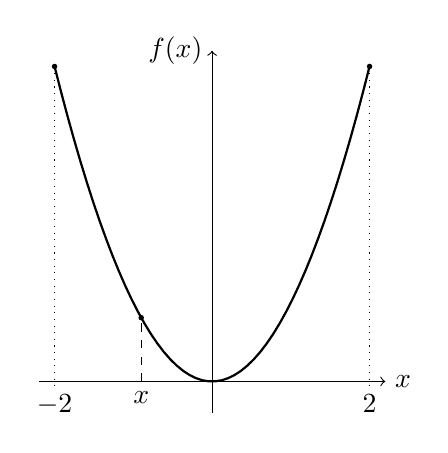
\begin{tikzpicture}\label{pagefuncaoquadratica}
\pgfmathsetmacro{\a}{2}
\fill (-\a,{\a^2}) circle (0.35mm);
\fill (\a,{\a^2}) circle (0.35mm);
\draw [thick, domain=-\a:\a, samples=50] plot (\x,{(\x)^2});
\draw [ ->] (-\a-0.2,0)--(\a+0.2,0) node[right]{$x$};
\draw [ ->] (0,-0.4)--(0,{\a^2+0.2}) node[left]{$f(x)$};
% \draw[thick] (-1,1)--(0,0)--(2,2);
\draw[dotted] ({-\a},{\a^2})--(-\a,-0.05) node[below]{$-2$};
\draw[dotted] (\a,{\a^2})--(\a,-0.05) node[below]{$2$};
%%%%%%%%%%
\pgfmathsetmacro{\x}{-0.9};
\pgfmathsetmacro{\y}{(\x)^2};
\draw (\x,0) node{$\shortmid$};
\draw (\x,0) node[below]{$x$};
\draw[dashed] (\x,0)--(\x,\y);
\fill (\x,\y) circle (0.35mm);
%%%%%%%%%%%
\end{tikzpicture}\end{bmlimage}
\end{center}
A curva obtida, chamada \grasA{parábola},\index{parábola} será usada inúmeras vezes nesse
curso.
\end{ex}

\begin{obs}
Um dos objetivos desse curso é de poder entender 
as principais propriedades de uma
função pelo estudo do seu gráfico. A noção de \emph{derivada} (ver Capítulo
\ref{Cap:Derivacao}) será de importância central nesse desenvolvimento.

No entanto, o gráfico da função $x^2$ acima foi feito com um computador. Primeiro,
o computador escolhe pontos entre $-2$ e $+2$, digamos $-2<x_1<\dots<x_n<2$, e calcula as  
posições $(x_j,f(x_j))$. Em seguida, ele traça a linha poligonal formada pelos segmentos
ligando $(x_j,f(x_j))$ a $(x_{j+1},f(x_{j+1}))$. Esse procedimento é chamado
\emph{interpolação}\index{interpolação}.
Por exemplo, escolhendo $n=3$, $5$ ou $9$ pontos no intervalo $[-2,2]$:
\begin{center}
\begin{bmlimage}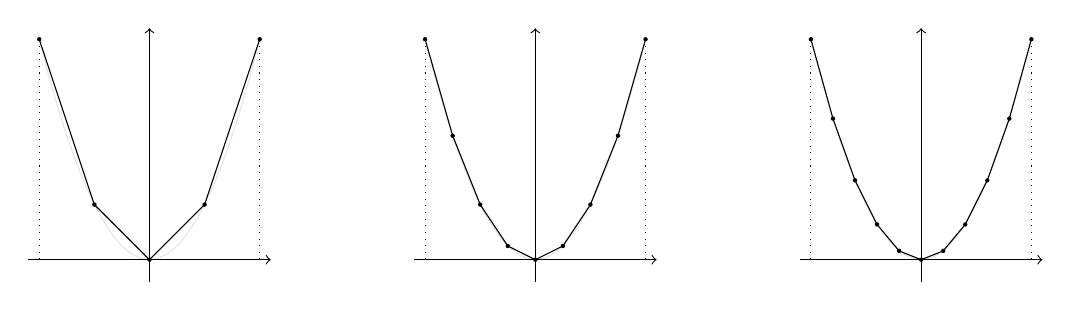
\begin{tikzpicture}[scale=0.7]
\pgfmathsetmacro{\a}{2}

\begin{scope}
\draw [thin, color=gray!20, domain=-\a:\a] plot (\x,{(\x)^2});
\newcommand{\funcao}[1]{((#1)^2)}
\draw [ ->] (-\a-0.2,0)--(\a+0.2,0);
\draw [ ->] (0,-0.4)--(0,{\a^2+0.2});
% \draw[thick] (-1,1)--(0,0)--(2,2);
\draw[dotted] ({-\a},{\a^2})--(-\a,-0.05);
\draw[dotted] (\a,{\a^2})--(\a,-0.05) ;
\pgfmathsetmacro{\l}{4};
\pgfmathsetmacro{\incr}{((2*\a)/(\l))};
\foreach \i in {1,...,\l} {
\fill ({(\i-1)*\incr-2},{\funcao{-2+(\i-1)*\incr}}) circle (0.40mm);
\draw ({-2+(\i-1)*(\incr)},{(-2+(\i-1)*(\incr))^2})--
({-2+(\i)*(\incr)},{(-2+(\i)*(\incr))^2});
}
\fill (2,4) circle (0.40mm);
\end{scope}

\begin{scope}[xshift=7cm]
\draw [thin, color=gray!20, domain=-\a:\a] plot (\x,{(\x)^2});
\draw [ ->] (-\a-0.2,0)--(\a+0.2,0);
\draw [ ->] (0,-0.4)--(0,{\a^2+0.2});
% \draw[thick] (-1,1)--(0,0)--(2,2);
\draw[dotted] ({-\a},{\a^2})--(-\a,-0.05) ;
\draw[dotted] (\a,{\a^2})--(\a,-0.05) ;
\pgfmathsetmacro{\k}{8};
\pgfmathsetmacro{\incr}{(2*\a/\k)};
\foreach \i in {1,...,\k} {
\fill ({-2+((\i)-1)*\incr},{(-2+(\i-1)*\incr)^2}) circle (0.40mm);
\draw ({-2+(\i-1)*\incr},{(-2+(\i-1)*\incr)^2})--
({-2+\i*\incr},{(-2+\i*\incr)^2});
}
\fill (2,4) circle (0.40mm);
\end{scope}

\begin{scope}[xshift=14cm]
\draw [thin, color=gray!20, domain=-\a:\a] plot (\x,{(\x)^2});
\draw [ ->] (-\a-0.2,0)--(\a+0.2,0);
\draw [ ->] (0,-0.4)--(0,{\a^2+0.2});
% \draw[thick] (-1,1)--(0,0)--(2,2);
\draw[dotted] ({-\a},{\a^2})--(-\a,-0.05) ;
\draw[dotted] (\a,{\a^2})--(\a,-0.05) ;
\pgfmathsetmacro{\k}{10};
\pgfmathsetmacro{\incr}{2*\a/\k};
\foreach \i in {1,...,\k} {
\fill ({-2+((\i)-1)*\incr},{(-2+(\i-1)*\incr)^2}) circle (0.40mm);
\draw ({-2+(\i-1)*\incr},{(-2+(\i-1)*\incr)^2})--
({-2+\i*\incr},{(-2+\i*\incr)^2});
}
\fill (2,4) circle (0.40mm);
\end{scope}

\end{tikzpicture}\end{bmlimage}
\end{center}
Quando o número de pontos escolhidos é grande e  
 $|x_{j+1}-x_j|$ é pequeno, a linha poligonal dá uma idéia do que deve ser o verdadeiro
esboço (o gráfico do Exemplo \ref{Ex:Grafxdois} foi feito com $n=50$, e já não dá mais
para perceber que a curva é na verdade uma linha poligonal).
O mesmo método permite (em princípio, tomando às vezes um certo cuidado) usar o computador
para esboçar o gráfico de qualquer função $f:D\mapsto \bR$.
Todos os gráficos dessa apostila foram feitos com esse método de interpolação. 
Enfatizemos que as ferramentas matemáticas desenvolvidas mais longe no curso 
permitirão extrair informações a respeito do
gráfico de uma função dada, \emph{sem} usar o computador. Isso será o objetivo do
\emph{estudo de funções}.
Lá, o computador poderá ser usado somente como meio de \emph{verificação}.
\end{obs}


Um problema inverso é de procurar uma função cujo esboço tenha características
específicas.
\begin{ex}
 Procuremos agora a função cujo gráfico é a metade superior do círculo de raio $R=4$
centrado na origem:\index{círculo! equação}
\begin{center}
\begin{bmlimage}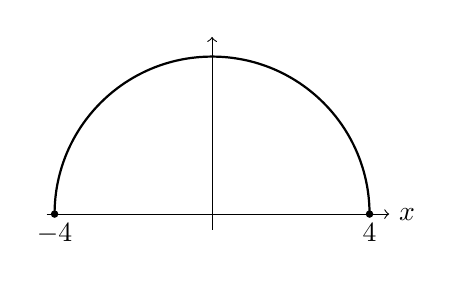
\begin{tikzpicture}[scale=0.5]
\pgfmathsetmacro{\a}{4}
%\draw [domain=-\a:\a] plot (\x,{sqrt(16-(\x)^2)});
\draw[thick] (4,0) arc (0:180:4);
\draw [ ->] (-\a-0.2,0)--(\a+0.5,0) node[right]{$x$};
\draw [ ->] (0,-0.4)--(0,{\a+0.5}) node[left]{};
% \draw[thick] (-1,1)--(0,0)--(2,2);
\draw (-\a,0) node[below]{$-4$};
\draw (\a,0) node[below]{$4$};
\fill (\a,0) circle (0.95mm);
\fill (-\a,0) circle (0.95mm);
\end{tikzpicture}\end{bmlimage}
\end{center}

 Lembre (Seção \ref{SecCirculos}) que o círculo \emph{completo} de raio $4$ centrado na
origem, $\gamma$, é formado pelos pontos $(x,y)$ tais que $x^2+y^2=16$. 
 A função procurada será obtida isolando $y$ nessa última relação. Para $y^2=16-x^2$ ter
soluções (aqui, $y$ é a incógnita), 
é preciso impor que $16-x^2\geq 0$, o que implica $-4\leq x\leq 4$. 
 Assim, o domínio da função procurada é $D=[-4,4]$ (como podia se adivinhar olhando para a
figura acima). 
 Assim, quando $x\in D$, a equação acima possui duas soluções $y=+\sqrt{16-x^2}$ e
$y=-\sqrt{16-x^2}$. Para selecionar o semi-círculo \emph{superior}, escolhamos a solução
positiva. Portanto, a função cujo gráfico é dado pelo semi-círculo acima é:
\begin{align*}
f:[-4,4]&\to\bR\\
x&\mapsto \sqrt{16-x^2}\,.
\end{align*}
\end{ex}

\begin{ex} Como a função ``valor absoluto'', funções podem ser definidas \emph{por
trechos}. Por exemplo, com $D=[-1,1)$, o gráfico da função
\begin{align*}
f(x)=
\begin{cases}
-x&\text{ se }-1\leq x< 0\,,\\
\sqrt{1-x^2}&\text{ se }0\leq x< 1\,,
\end{cases}
\end{align*}
é formado pela reta de inclinação $m=-1$ que passa pela origem
entre $x=-1$ e $x=0$, e pela parte do semi-círculo de raio $1$ centrado na origem 
entre $x=0$ e $x=1$:
\begin{center}
\begin{bmlimage}\begin{tikzpicture}
\pgfmathsetmacro{\a}{1}
%\draw [domain=-\a:\a] plot (\x,{sqrt(16-(\x)^2)});
\draw[thick] (0,1) arc (90:0:1);
\draw [->] (-\a-0.2,0)--(\a+0.3,0) node[right]{$x$};
\draw [->] (0,-0.4)--(0,{\a+0.3}) node[left]{};
\draw[thick] (-1,1)--(0,0);
\fill (0,1) circle (0.45mm);
\fill (-1,1) circle (0.45mm);
\fill[intaberto] (0,0) circle (0.45mm);
\fill[intaberto] (1,0) circle (0.45mm);
\draw (-\a,0) node{$\shortmid$};
\draw (-\a,0) node[below]{$-1$};
\draw (\a,0) node[below]{$1$};
\end{tikzpicture}\end{bmlimage}
\end{center}
 Observe que essa função possui uma \emph{descontinuidade em $x=0$}: ao variar $x$ entre
pequenos valores $x<0$ e pequenos valores $x>0$, $f(x)$ pula de valores perto de zero para
valores perto de $1$. 
\end{ex}

\begin{exo}
Dê uma função (e o seu domínio) cujo gráfico seja:
\begin{enumerate}
\item \label{itgrafunc0} a reta horizontal que passa pelo ponto $(-21,-1)$
\item\label{itgrafunc1} a parte inferior do círculo de raio $9$ centrado 
em $(5,-4)$ 
\item \label{itgrafunc2} a parte do círculo de raio $5$ centrado na 
origem que fica
estritamente acima da reta de equação $y=3$
\item \label{itgrafunc3} a parte do círculo de raio $5$ centrado na 
origem contida no quarto quadrante
\end{enumerate}
\vspace{0.01cm}
\begin{sol}
\eqref{itgrafunc0} $f(x)=-1$, $D=\bR$
\eqref{itgrafunc1} $f(x)=-\sqrt{81-(x-5)^2}-4$, $D=[-4,14]$.
\eqref{itgrafunc2} $f(x)=\sqrt{25-x^2}$, $D=(-4,4)$
\eqref{itgrafunc3} $f(x)=-\sqrt{25-x^2}$, $D=[0,5]$
\end{sol}
\end{exo}

\begin{exo}\label{ExoEsbocosElementares}
Esboce os gráficos das seguintes funções (todas com $D=\bR$):
\begin{enumerate}
\item $f(x)= 1$ se $x\leq 1$, $f(x)=x^2$ caso contrário,
\item $g(x)=-|x-1|$,
\item $h(x)=\lfloor x\rfloor$,
\item $i(x)=x-\lfloor x\rfloor$,
\item $j(x)=||x|-1|$.
\end{enumerate}
\vspace{0.01cm}
\begin{sol}\mbox{}

\begin{bmlimage}\begin{tikzpicture}
\begin{scope}[xshift=-0.5cm]
\draw[thick] (-0.7,1)--(1,1);
\fill (1,1) circle (0.45mm);
\draw [thick, domain=1:1.5] plot (\x,{(\x)^2});
\draw [ ->] (-1.2,0)--(1.2,0);
\draw [ ->] (0,-0.4)--(0,{1.2});
\draw (0,1) node[right]{$1$};
\draw (-0.5,0.5) node{$f(x)$};
\end{scope}

\begin{scope}[xshift=1.8cm, yshift=1cm]
\draw [ ->] (-0.2,0)--(2.2,0);
\draw [ ->] (0,-1)--(0,0.5);
\draw (0,0.4) node[right]{$g(x)$};
\draw (1,0) node[above]{$1$};
\draw[thick] (0.2,-0.8)--(1,0)--(2,-1);
\end{scope}

\begin{scope}[xshift=5.8cm, yshift=0.5cm]
\draw [ ->] (-1.5,0)--(1.5,0);
\draw [ ->] (0,-1)--(0,1);
\draw (0,0.8) node[left]{$h(x)$};
\foreach \k in {-3,...,3}{
\pgfmathsetmacro{\a}{\k/3};
\fill (\a,\a) circle (0.45mm);
\draw[thick] (\a,\a)--({\a+0.333},\a);
\fill[intaberto] ({\a+0.333},\a) circle (0.45mm);
}
\end{scope}

\begin{scope}[xshift=9cm, yshift=0.5cm]
\draw [ ->] (-1.3,0)--(1.3,0);
\draw [ ->] (0,-1)--(0,1);
\draw (0,0.8) node[left]{$i(x)$};
\foreach \k in {-3,...,3}{
\pgfmathsetmacro{\a}{\k/3};
\fill (\a,0) circle (0.45mm);
\draw[thick] (\a,0)--({\a+0.333},0.333);
\fill[intaberto] ({\a+0.333},0.333) circle (0.45mm);
}
\end{scope}

\begin{scope}[xshift=12.5cm, yshift=0.1cm, scale=0.7]
\draw [ ->] (-1.3,0)--(1.3,0);
\draw [ ->] (0,-0.3)--(0,1.3) node[left]{$j(x)$};
%\draw [thick, domain=-1.5:1.5, samples=20] plot (\x,{abs(abs(\x)-1)});
\draw[thick] (-2.2,1.2)--(-1,0)--(0,1)--(1,0)--(2.2,1.2);
\end{scope}

\end{tikzpicture}\end{bmlimage}
\end{sol}
\end{exo}


\begin{exo}
Determine quais curvas abaixo são (ou não são) gráficos de funções. Quando for um gráfico,
dê a função associada.
\begin{center}
\begin{bmlimage}\begin{tikzpicture}
 \begin{scope}
\draw[thick] (-1.2,-1)--(1,-1);
\fill (1,-1) circle (0.45mm);
\draw [thick] (1,1)--(2.5,-0.5);
\fill[intaberto] (1,1) circle (0.45mm);
%\draw [thick,  <-, domain=0:1] plot (\x,{(\x)^2});
\draw [ ->] (-1.2,0)--(3,0);
\draw [ ->] (0,-1.2)--(0,{1.2});
\draw (1,0) node{$\shortmid$};
\draw (1,0) node[above left]{$1$};
\end{scope}

\begin{scope}[xshift=5.5cm]
\fill (0,-1) circle (0.45mm);
\draw [thick, domain=-1.2:0] plot (\x,{-sqrt(1-\x)});
\draw [thick, domain=-1.2:0] plot (\x,{-sqrt(1-\x)});
\draw [->] (-1.2,0)--(1.2,0);
\draw [thick, domain=-0.5:1.2] plot (\x,{sqrt(\x+1)});
\draw[dotted] (-0.5,0)--(-0.5,{sqrt(-0.5+1)});
\draw [->] (0,-1.3)--(0,{1.3});
\fill[intaberto] (-0.5,0.707) circle (0.45mm);
\draw (-0.5,0) node[below]{$\scriptstyle{-\tfrac12}$};
\end{scope}

\begin{scope}[xshift=10cm]
\draw [ ->] (-2.4,0)--(2.4,0);
\draw [ ->] (0,-0.8)--(0,{1.3});
\foreach \i in {-2,-1,0,1} {
\draw[thick] (\i,1)--(\i+1,1);
\fill[intaberto] (\i,1) circle (0.45mm);
}
\foreach \i in {-2,-1,0,1,2} {
\draw[dotted] (\i,0)--(\i,1);
\fill (\i,0) circle (0.45mm);
\draw (\i,0) node[below]{$\i$};
}
\end{scope}

\end{tikzpicture}\end{bmlimage}
\end{center}
\begin{sol}
A primeira curva é o gráfico da função $f(x)=-1$ se $x\leq 1$, $f(x)=2-x$ se $x>1$. 
 A segunda não é um gráfico, pois os pontos $-\tfrac12 <x\leq 0$ têm duas saídas, o que
não é descrito por uma função (lembra que uma função é um mecanismo que a um entrada $x$
do domínio associa \emph{um (único)} número $f(x)$). No entanto, seria possível
interpretar aquela curva como a união dos gráficos de duas funções distintas: uma função 
$f$ com domínio $(-\infty,0]$, e uma outra função $g$ com domínio $(-\tfrac12,\infty)$.
A terceira é o gráfico da função $f(x)=0$ se $x\in \bZ$, $f(x)=1$ caso contrário.
\end{sol}
\end{exo}

\subsection{Potências inteiras: $x^p$}\label{Sec:GraficosPotencias}
 Já esboçamos o gráfico da função $f(x)=x^2$ no Exemplo \ref{Ex:Grafxdois}. Vejamos agora
o caso mais geral de uma potência $f(x)=x^p$, onde $p\in \bZ$ (excluiremos o caso $p=0$,
que corresponde a $f(x)=1$). 

\subsubsection{Potências positivas}\index{potência! inteira, positiva}
Para potências positivas \emph{inteiras}, $p>0$, temos $x^p=x\cdot x\cdots x$ ($p$ vezes),
logo o domínio de $x^p$ é sempre $D=\bR$.
Quando $p$ é positiva e \grasA{par}, isto é, $p\in \{ 2,4,6, \dots\}$, então 
$x^p\geq 0$ para todo $x$, e os gráficos são da forma:
\begin{center}
\begin{bmlimage}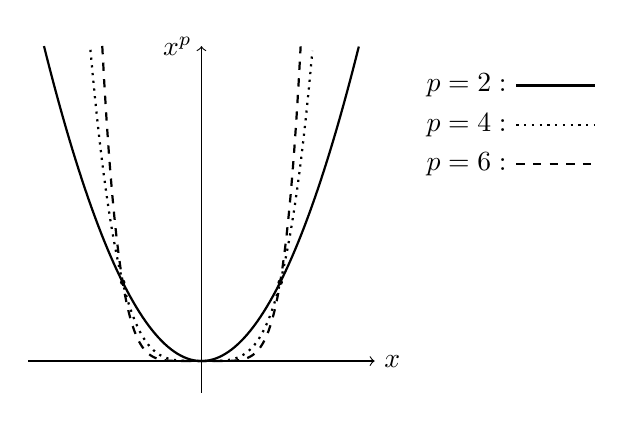
\begin{tikzpicture}[scale=1]
\pgfmathsetmacro{\a}{1.41}
\draw [thick, dotted, domain=-\a:\a, samples=100] plot
(\x,{(\x)^4});
\pgfmathsetmacro{\a}{1.26}
\draw [thick, dashed, domain=-\a:\a, samples=100] plot
(\x,{(\x)^6});
\pgfmathsetmacro{\a}{2}
\draw [thick, domain=-\a:\a, samples=100] plot (\x,{(\x)^2});
\fill (-1,1) circle (0.35mm);
\fill (1,1) circle (0.35mm);
\draw [ ->] (-2.2,0)--(2.2,0) node[right]{$x$};
\draw [ ->] (0,-0.4)--(0,{4}) node[left]{$x^p$};
\pgfmathsetmacro{\b}{4};
\pgfmathsetmacro{\c}{3.5};
\draw (\b,\c) node[left]{$p=2:$};
\draw[thick] (\b,\c)--(\b+1,\c);
\draw (\b,\c-0.5) node[left]{$p=4:$};
\draw[thick, dotted] (\b,\c-0.5)--(\b+1,\c-0.5);
\draw (\b,\c-1) node[left]{$p=6:$};
\draw[thick, dashed] (\b,\c-1)--(\b+1,\c-1);
\end{tikzpicture}\end{bmlimage}
\end{center}
 Observe que todos os gráficos passam pela origem e pelos pontos 
 $(-1,1)$ e $(1,1)$, e que as funções correspondentes não são 
 limitadas superiormente: tomam 
valores arbitrariamente grandes longe da 
origem (no entanto, todas são limitadas inferiormente por $M_-=0$). 
Vemos
também que quanto maior o $p$, mais rápido $x^p$ cresce quando $x$
cresce.\\

 Quando a potência $p$ é positiva e \grasA{ímpar}, isto é, $p\in \{ 1,3,5, \dots\}$, então
há uma mudança de sinal:
$x^p\geq 0$ para $x\geq 0$, $x^p\leq 0$ para $x\leq 0$. Os gráficos são da forma:
\begin{center}
\begin{bmlimage}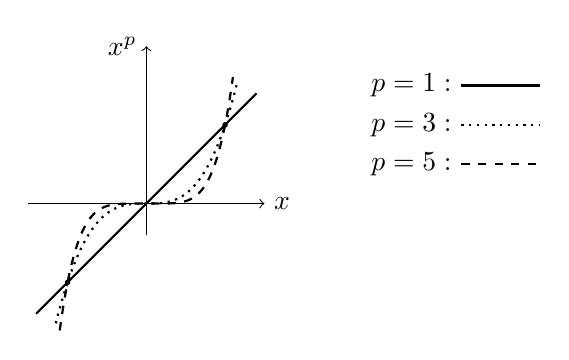
\begin{tikzpicture}[scale=1]
\pgfmathsetmacro{\a}{1.15}
\draw [thick, dotted, domain=-\a:\a, samples=100] plot (\x,{\x^3});
\pgfmathsetmacro{\a}{1.1}
\draw [thick, dashed, domain=-\a:\a, samples=100] plot (\x,{\x^5});
\pgfmathsetmacro{\a}{1.4}
\draw [thick, domain=-\a:\a, samples=100] plot (\x,{\x});
\fill (1,1) circle (0.35mm);
\fill (-1,-1) circle (0.35mm);
\draw [ ->] (-1.5,0)--(1.5,0) node[right]{$x$};
\draw [ ->] (0,-0.4)--(0,{2}) node[left]{$x^p$};
\pgfmathsetmacro{\b}{4};
\pgfmathsetmacro{\c}{1.5};
\draw (\b,\c) node[left]{$p=1:$};
\draw[thick] (\b,\c)--(\b+1,\c);
\draw (\b,\c-0.5) node[left]{$p=3:$};
\draw[thick, dotted] (\b,\c-0.5)--(\b+1,\c-0.5);
\draw (\b,\c-1) node[left]{$p=5:$};
\draw[thick, dashed] (\b,\c-1)--(\b+1,\c-1);
\end{tikzpicture}\end{bmlimage}
\end{center}
Observe que nenhuma dessas funções é limitada em $\bR\backslash\{0\}$, 
nem inferiormente nem superiormente.

\subsubsection{Potências negativas}\label{Subsec:graficpotnegativ}\index{potência!
inteira, negativa}
A potência negativa $p={-1}$ já foi encontrada no Exemplo \ref{Ex:Umsobrex}.
Se $p<0$, escreveremos $p=-q$ com $q>0$. Assim, $x^p=\tfrac{1}{x^q}$, que não é definida em $x=0$:
\begin{align*}
 f:\bR\setminus\{0\}&\to\bR\\
x&\mapsto \tfrac{1}{x^q}
\end{align*}
Quando a potência $q$ é \grasA{par}, isto é, $q\in \{ 2,4,6, \dots\}$, então 
$\tfrac{1}{x^{q}}\geq 0$ para todo $x\neq 0$, e os gráficos são da forma:
\begin{center}
\begin{bmlimage}\begin{tikzpicture}[scale=1]
\pgfmathsetmacro{\a}{4}

\draw [thick, domain=-\a:-0.5, samples=100] plot (\x,{1/((\x)^2)});
\draw [thick, domain=0.5:\a, samples=100] plot  (\x,{1/((\x)^2)});

\draw [thick, dotted, domain=-\a:-0.72, samples=100] plot
(\x,{1/((\x)^4)});
\draw [thick, dotted, domain=0.72:\a, samples=100] plot (\x,{1/((\x)^4)});

\draw [thick, dashed, domain=-\a:-0.8, samples=100] plot
(\x,{1/((\x)^6)});
\draw [thick, dashed, domain=0.8:\a, samples=100] plot (\x,{1/((\x)^6)});

\draw [ ->] (-4,0)--(4,0) node[right]{$x$};
\draw [ ->] (0,-0.4)--(0,{3}) node[above]{$\tfrac{1}{x^q}$};
 \pgfmathsetmacro{\b}{4};
 \pgfmathsetmacro{\c}{3.5};
 \draw (\b,\c) node[left]{$q=2:$};
 \draw[thick] (\b,\c)--(\b+1,\c);
 \draw (\b,\c-0.5) node[left]{$q=4:$};
 \draw[thick, dotted] (\b,\c-0.5)--(\b+1,\c-0.5);
 \draw (\b,\c-1) node[left]{$q=6:$};
 \draw[thick, dashed] (\b,\c-1)--(\b+1,\c-1);
\end{tikzpicture}\end{bmlimage}
\end{center}
 Observe que para cada uma dessas funções, ao $x$ se aproximar de $0$, $f(x)$ cresce e
toma valores arbitrariamente \emph{grandes}: é não-limitada. Diremos (mais tarde) que
 há uma \emph{assíntota vertical} em $x=0$. 
Também, quando $x$ toma valores grandes, $f(x)$ decresce e toma 
valores arbitrariamente \emph{pertos de zero}. Diremos (mais tarde) que a função
\emph{tende a zero no infinito}, e que a reta horizontal $y=0$
é \emph{assíntota horizontal}.\\

 Quando a potência é \grasA{ímpar}, a mesma mudança de sinal acontece, e os gráficos têm
propriedades parecidas:
\begin{center}
\begin{bmlimage}\begin{tikzpicture}[scale=1]
\pgfmathsetmacro{\a}{4}

\draw [thick, domain=-\a:-0.32, samples=100] plot (\x,{1/((\x))});
\draw [thick, domain=0.32:\a, samples=100] plot (\x,{1/((\x))});

\draw [thick, dotted, domain=-\a:-0.72, samples=100] plot
(\x,{1/((\x)^3)});
\draw [thick, dotted, domain=0.72:\a, samples=100] plot (\x,{1/((\x)^3)});

\draw [thick, dashed, domain=-\a:-0.8, samples=100] plot
(\x,{1/((\x)^5)});
\draw [thick, dashed, domain=0.8:\a, samples=100] plot (\x,{1/((\x)^5)});

\draw [ ->] (-4,0)--(4,0) node[right]{$x$};
\draw [ ->] (0,-3)--(0,{3}) node[above]{$\tfrac{1}{x^q}$};
 \pgfmathsetmacro{\b}{4};
 \pgfmathsetmacro{\c}{3.5};
 \draw (\b,\c) node[left]{$q=1:$};
 \draw[thick] (\b,\c)--(\b+1,\c);
 \draw (\b,\c-0.5) node[left]{$q=3:$};
 \draw[thick, dotted] (\b,\c-0.5)--(\b+1,\c-0.5);
 \draw (\b,\c-1) node[left]{$q=5:$};
 \draw[thick, dashed] (\b,\c-1)--(\b+1,\c-1);
\end{tikzpicture}\end{bmlimage}
\end{center}

\subsection{Paridade}

Observemos algumas simetrias nos gráficos das funções $x^p$ da seção anterior.
 Primeiro, para os valores de $p$ \emph{pares}, o gráfico de $x^p$ é \emph{simétrico com
respeito ao eixo $y$}, o que segue do seguinte fato: $(-x)^p=x^p$. 
 Por outro lado, para os valores de $p$ \emph{ímpares}, o gráfico de $x^p$ é
\emph{simétrico com respeito à origem} (por uma rotação de $180^o$), o que segue do fato
seguinte: $(-x)^p=-x^p$. \\

Esses fatos \index{função! par}\index{função! par} 
levam a introduzir duas noções gerais. Por um lado, diremos que
$$\boxed{\text{$f$ é \grasA{par} se }f(-x)=f(x)\,,\quad\forall x\text{
do seu domínio.}}$$
Por outro lado,
$$\boxed{\text{$f$ é \grasA{impar} se }f(-x)=-f(x)\,,\quad\forall x\text{
do seu domínio.}}$$ 
\begin{ex}
A função $f(x)=\frac{x^2}{1-x^4}$ é par. De fato, como as potências
envolvidas são pares, $(-x)^2=x^2$, $(-x)^4=x^4$, assim:
$$
f(-x)=\frac{(-x)^2}{1-(-x)^4}=\frac{x^2}{1-x^4}=f(x)\,.
$$
\end{ex}

\begin{ex}
Considere $g(x)=\frac{x^2}{\sen (x)}$.
Vimos que o seno é uma função ímpar: $\sen(-x)=-\sen x$. 
Como consequência, a função $g$ é ímpar, já que
\[
g(-x)=\frac{(-x)^2}{\sen(-x)}=\frac{x^2}{-\sen x}=
-\frac{x^2}{\sen x}=-g(x)\,.
\]
\end{ex}
Mas uma função, em geral, não precisa ser par ou ímpar.
Para mostrar que uma função $f$ não é par, basta achar um ponto
$x$ em que $f(-x)\neq f(x)$. Do mesmo jeito, para mostrar que $f$ não é ímpar, basta achar um ponto em
que $f(-x)\neq -f(x)$.
\begin{ex}
Mostremos que $f(x)=x+1$ não é par. 
De fato, olhando para o ponto $x=-1$, temos $f(-1)=0$, e $f(1)=2$. Logo,
$f(-1)\neq f(1)$. Mas como $f(-1)\neq -f(1)$, $f$ também não é ímpar.
\end{ex}

\begin{exo}
Determine quais das funções $f$ abaixo são pares ou ímpares (justificando a sua
resposta). Quando não for nem par nem ímpar, dê um contra-exemplo.
\begin{multicols}{4}
\begin{enumerate}
\item\label{itparidade1} $\tfrac{x}{x^3-x^5}$
\item\label{itparidade2} $\sqrt{1-x^2}$
\item\label{itparidade3} $x^2\sen x$
\item\label{itparidade4} $\sen (\cos x)$
\item\label{itparidade41} $\sen (\sen x)$
\item\label{itparidade5} $\sen^2 x-\cos x$
\item\label{itparidade6} $\sen x+\cos x$
\item\label{itparidade7} $\sqrt{x^2}-|x|$
\end{enumerate}
\end{multicols}
\vspace{0.01cm}
\begin{sol}
\eqref{itparidade1} É par: $f(-x)=\tfrac{(-x)}{(-x)^3-(-x)^5}=\tfrac{-x}{-(x^3-x^5)}=f(x)$.
\eqref{itparidade2} É par: $f(-x)=\sqrt{1-(-x)^2}=\sqrt{1-x^2}=f(x)$.
\eqref{itparidade3} É ímpar: $f(-x)=(-x)^2\sen (-x)=x^2(-\sen x)=-f(x)$.
\eqref{itparidade4} É par: $f(-x)=\sen (\cos(-x))=\sen(\cos x)=f(x)$.
\eqref{itparidade41} É ímpar: $f(-x)=\sen (\sen(-x))=\sen(-\sen x)=-\sen(\sen x)=-f(x)$.
\eqref{itparidade5} É par: $f(-x)=(\sen(-x))^2-\cos(-x)=(-\sen x)^2-\cos x=f(x)$.
 \eqref{itparidade6} Não é par nem ímpar, pois $f(\pisobrequatro)=\sqrt{2}$,
$f(-\pisobrequatro)=0$.
\eqref{itparidade7} Como $f(x)\equiv 0$, ela é par \emph{e} ímpar.
\end{sol}
\end{exo}


\subsection{Crescimento e decrescimento}\label{sec_Funcoes_variacao}
O que mais nos interessará, no estudo de uma função $f$ dada,
será distinguir as regiões em que ela \emph{cresce/decresce}:

\begin{defin} Seja $I$ um intervalo.
Uma função $f$ é \index{função!crescente}
\begin{itemize}
 \item \grasA{crescente em $I$} se $f(x)\leq f(x')$ para todo $x,x'\in
 I$, $x<x'$.
\item \grasA{estritamente crescente em $I$} se $f(x)<  f(x')$ para todo $x,x'\in
 I$, $x< x'$.\index{função!decrescente}
 \item \grasA{decrescente em $I$} se $f(x)\geq f(x')$ para todo $x,x'\in
 I$, $x< x'$.
\item \grasA{estritamente decrescente em $I$} se $f(x)>  f(x')$ para todo $x,x'\in
 I$, $x< x'$.
\end{itemize}
\end{defin}

Por exemplo, o gráfico de uma função estritamente crescente:
\begin{center}
\begin{bmlimage}\begin{tikzpicture}
\pgfmathsetmacro{\a}{1}
\pgfmathsetmacro{\b}{3}
\newcommand{\mafonc}[1]{4-0.2*( #1 -5)^2}
\draw [thick, domain=0:4.5, samples=100] plot (\x,{\mafonc{\x}});
\draw [ ->] (-0.1,0)--(4,0);
\draw [ ->] (0,-0.5)--(0,{4.5});
\draw[dashed] (\a,0) node[below]{$x$}--(\a,{\mafonc{\a}})--(0,{\mafonc{\a}}) node[left]{$f(x)$};
\draw[dashed] (\b,0) node[below]{$x'$}--(\b,{\mafonc{\b}})--(0,{\mafonc{\b}}) node[left]{$f(x')$};
\end{tikzpicture}\end{bmlimage}
\end{center}
Pela definição acima, uma função constante é ao mesmo tempo crescente e decrescente.\\

\grasA{Estudar a variação} de uma função $f$ será entendido como \emph{procurar
os intervalos em que $f$ cresce ou decresce}. 

\begin{exo}
Estude a variação das funções abaixo.
\begin{multicols}{4}
\begin{enumerate}
\item\label{itexodecr1} $x$
\item \label{itexodecr2}$|x|$
\item \label{itexodecr3}$x^2$
\item \label{itexodecr4}$x^3$
\item \label{itexodecr5}$\frac{1}{x}$
\item \label{itexodecr6}$\frac{1}{x^2}$
\item \label{itexodecr7}$x-x^2$
\item \label{itexodecr8}$||x|-1|$
\end{enumerate}
\end{multicols}
\vspace{0.05cm}
\begin{sol}
\eqref{itexodecr1} cresce na reta toda.
\eqref{itexodecr2} decrescce (estritamente) em $(-\infty,0]$, cresce (estritamente) em $[0,\infty)$.
\eqref{itexodecr3} decrescce (estritamente) em $(-\infty,0]$, cresce (estritamente) em $[0,\infty)$.
\eqref{itexodecr4}  cresce (estritamente) na reta toda.
\eqref{itexodecr5} decrescce (estritamente) em $(-\infty,0)$, decresce (estritamente) em $(0,\infty)$.
\eqref{itexodecr6} crescce (estritamente) em $(-\infty,0)$, decresce (estritamente) em $(0,\infty)$.
\eqref{itexodecr7} crescce (estritamente) em $(-\infty,\tfrac12]$, decresce (estritamente) em
$[\tfrac12,\infty$. (Será mais fácil resolver esse item depois de saber esboçar o gráfico de $x-x^2$,
veja o Exemplo \ref{exemplo_Funcoes_grafparabdesloc}.)
\eqref{itexodecr8} decrescce (estritamente) em $(-\infty,-1]$ e em $[0,1]$, 
cresce (estritamente) em $[-1,0]$ e $[1,\infty)$.
\end{sol}
\end{exo}

Mais tarde introduziremos uma ferramenta fundamental (a \emph{derivada}) para o estudo da variação.

\subsection{Funções Trigonométricas}\label{Sec:GraficosTrigo}
Começemos com o gráfico de $\sen x$, para $x\in [0,2\pi]$:\index{seno! gráfico}

\begin{center}
\begin{bmlimage}\begin{tikzpicture}

\begin{scope}[scale=0.7]
\pgfmathsetmacro{\a}{2.3};
\draw (-\a,0) -- (0,0);
\draw[ ->] (0,-\a) -- (0,\a);
\draw[ ->] (1.1,0)-- (\a,0);
\draw (0,0)--(1 r:2);
\draw [color=\coulseno, thick] (1.1,1.665)--(1.1,0) node[midway, above, sloped]{$\sen x$};
\draw[dotted] (2,0) arc (0:360:2);
\draw (0,0)--(2,0);
\draw (0.5,1.1) node{$1$};
\draw[->] (0.5,0) arc (0:1 r:0.5);
\draw (0.4,0.3) node[right]{$x$};
\fill (1.1,1.665) circle (0.45mm);
\draw (4,0) node{$\Rightarrow$};
\end{scope}

\begin{scope}[scale=1.2, xshift=3.5cm]
\draw [thick, domain=0:6.28, samples=100] plot (\x,{sin(\x r)});
\draw [ ->] (-0.2,0)--(7,0) node[right]{$x$};
\draw [ ->] (0,-1.3)--(0,{1.3}) node[right]{$\sen x$};
\draw[thick, color=\coulseno] (1,{sin(1 r)})--(1,0) node[midway, above, sloped]{$\sen x$};
\fill (1,{sin(1 r)}) circle (0.28mm);
\draw (1,0) node{$\shortmid$};
\draw (1,0) node[below]{$x$};
\draw[dotted] (0,1)--(6.28,1);
\draw (0,1) node[left]{$1$};
\draw[dotted] (0,-1)--(6.28,-1);
\draw (0,-1) node[left]{$-1$};
\draw (3.14,0) node{$\shortmid$};
\draw (3.15,0) node[above]{$\pi$};
\draw (6.28,0) node{$\shortmid$};
\draw (6.28,0) node[above]{$2\pi$};
\end{scope}
\end{tikzpicture}\end{bmlimage}
\end{center}
Se o seno for considerado na reta real toda, obtemos:
\begin{center}
 \begin{bmlimage}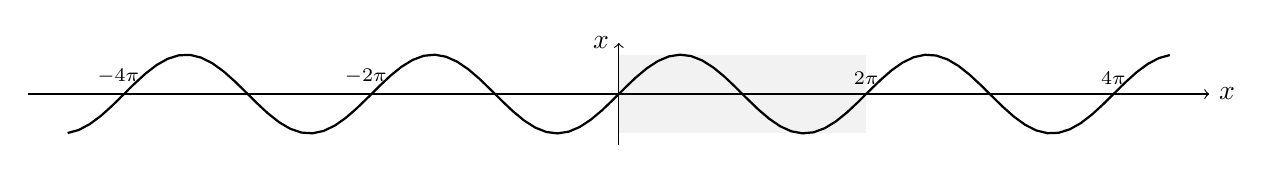
\begin{tikzpicture}[scale=0.5]
\fill[color=gray!10] (0,-1) rectangle (6.28,1);
  \draw [thick, domain=-14:14, samples=100] plot (\x,{sin(\x r)});
\draw [ ->] (-15,0)--(15,0) node[right]{$x$};
\draw [ ->] (0,-1.3)--(0,{1.3}) node[left]{$\sen x$};
\pgfmathsetmacro{\Pi}{3.1415};
\draw ({-4*\Pi},0) node[above]{$\scriptstyle{ -4\pi}\,\,\,$};
\draw ({-4*\Pi},0) node{$\shortmid$};
\draw ({-2*\Pi},0) node[above]{$\scriptstyle{ -2\pi}\,\,\,$};
\draw ({-2*\Pi},0) node{$\shortmid$};
\draw ({2*\Pi},0) node[above]{$\scriptstyle{ 2\pi}$};
\draw ({2*\Pi},0) node{$\shortmid$};
\draw ({4*\Pi},0) node[above]{$\scriptstyle{4\pi}$};
\draw ({4*\Pi},0) node{$\shortmid$};
 \end{tikzpicture}\end{bmlimage}
\end{center}
 Observemos que esse gráfico é simétrico em torno da origem (por uma
 rotação de $\pi$), o que
 reflete o fato do seno ser uma função ímpar. Vemos também que $\sen$ é
\grasA{periódica}\index{função! periódica}, de período $2\pi$\index{período}:
$$\boxed{\sen (x+2\pi)=\sen x\,,\quad \forall x\in \bR\,.}$$
Geometricamente: o gráfico completo (para $x\in \bR$) 
é obtido usando translações do gráfico da figura anterior (hachurado, feito para $x\in
[0,2\pi]$).
Essa propriedade pode ser provada analiticamente, usando \eqref{eqtrigo000}:
$\sen(x+2\pi)=\sen(\pi+(x+\pi))=-\sen(x+\pi)=\sen x$.\\

Considerações análogas se aplicam ao cosseno:\index{cosseno! gráfico}

\begin{center}
\begin{bmlimage}\begin{tikzpicture}

\begin{scope}[scale=0.7]
\pgfmathsetmacro{\a}{2.3};
\draw (-\a,0) -- (0,0);
\draw[ ->] (0,-\a) -- (0,\a);
\draw[ ->] (1.1,0)-- (\a,0);
\draw (0,0)--(1 r:2);
\draw [color=\coulcoseno, thick] (1.1,0)--(0,0) node[midway, below]{$\cos x$};
\draw[dotted] (1.1,0)--(1.1,1.665);
\draw[dotted] (2,0) arc (0:360:2);
\draw (1.1,0)--(2,0);
\draw (0.5,1.1) node{$1$};
\draw[->] (0.5,0) arc (0:1 r:0.5);
\draw (0.4,0.3) node[right]{$x$};
\fill (1.1,1.665) circle (0.45mm);
\draw (4,0) node{$\Rightarrow$};
\end{scope}

\begin{scope}[scale=1.2, xshift=3.5cm]
\draw [thick, domain=0:6.28, samples=100] plot (\x,{cos(\x r)});
% \draw[thick] (1,0) arc (0:90:1);
\draw [ ->] (-0.2,0)--(7,0) node[right]{$x$};
\draw [ ->] (0,-1.3)--(0,{1.3}) node[right]{$\cos x$};
% \fill (0,1) circle (0.45mm);
\draw[thick, color=\coulcoseno] (1,{cos(1 r)})--(1,0) node[midway, below, sloped]{$\cos x$};
\fill (1,{cos(1 r)}) circle (0.28mm);
\draw (1,0) node{$\shortmid$};
\draw (1,0) node[below]{$x$};
\draw[dotted] (0,1)--(6.28,1);
\draw (0,1) node[left]{$1$};
\draw[dotted] (0,-1)--(6.28,-1);
\draw (0,-1) node[left]{$-1$};
\draw (3.14,0) node{$\shortmid$};
\draw (3.15,0) node[above]{$\pi$};
\draw (6.28,0) node{$\shortmid$};
\draw (6.28,0) node[above]{$2\pi$};
\end{scope}
\end{tikzpicture}\end{bmlimage}
\end{center}
Quando considerado na reta real, o cosseno é par, e também tem período $2\pi$:
\begin{center}
 \begin{bmlimage}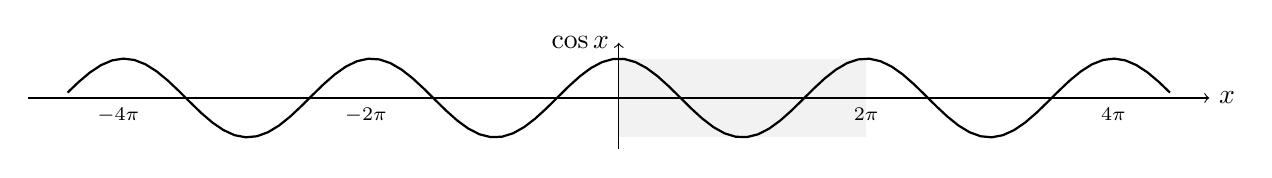
\begin{tikzpicture}[scale=0.5]
\fill[color=gray!10] (0,-1) rectangle (6.28,1);
  \draw [thick, domain=-14:14, samples=100] plot (\x,{cos(\x r)});
\draw [ ->] (-15,0)--(15,0) node[right]{$x$};
\draw [ ->] (0,-1.3)--(0,{1.4}) node[left]{$\cos x$};
\pgfmathsetmacro{\Pi}{3.1415};
\draw ({-4*\Pi},0) node[below]{$\scriptstyle{ -4\pi}\,\,\,$};
\draw ({-4*\Pi},0) node{$\shortmid$};
\draw ({-2*\Pi},0) node[below]{$\scriptstyle{ -2\pi}\,\,\,$};
\draw ({-2*\Pi},0) node{$\shortmid$};
\draw ({2*\Pi},0) node[below]{$\scriptstyle{ 2\pi}$};
\draw ({2*\Pi},0) node{$\shortmid$};
\draw ({4*\Pi},0) node[below]{$\scriptstyle{4\pi}$};
\draw ({4*\Pi},0) node{$\shortmid$};
 \end{tikzpicture}\end{bmlimage}
\end{center}

O esboço da função tangente é um pouco mais delicado. Como foi visto no início do capítulo, 
$\tan x=\frac{\sen x}{\cos x}$ é bem definida somente se $x$ é diferente de $\tfrac{\pi}{2}\pm k\pi$.
Isso implica a presença de \emph{assíntotas verticais} no gráfico:\index{tangente!
gráfico}

\begin{center}
\begin{bmlimage}\begin{tikzpicture}

\begin{scope}[scale=0.7]
\pgfmathsetmacro{\a}{2.3};
\draw (-\a,0) -- (0,0);
\draw[ ->] (0,-\a) -- (0,\a);
\draw[ ->] (1.1,0)-- (\a,0);
%\draw (0,0)--(1 r:2);
%\draw [color=\coulseno, thick] (1.1,1.665)--(1.1,0) node[midway, above, sloped]{$\sen x$};
 \draw [color=\coultang, thick] (2,3)--(2,0) node[midway, above, sloped]{$\tan x$};
%\draw [color=coulcoseno, thick] (1.1,0)--(0,0) node[midway, below]{$\cos x$};
% \draw (1.1,1.665) node[above]{$B$};
%\draw[dotted] (1.1,0)--(1.1,1.665);
\draw[dotted] (2,0) arc (0:360:2);
\draw(0,0)--(2,3);
\draw (0,0)--(2,0);
\draw (0.5,1.1) node{$1$};
\draw[->] (0.5,0) arc (0:1 r:0.5);
\draw (0.4,0.3) node[right]{$x$};
\fill (1.1,1.665) circle (0.45mm);
\draw (4,0) node{$\Rightarrow$};
\end{scope}

\pgfmathsetmacro{\eps}{0.3};
\pgfmathsetmacro{\pisd}{1.5707};
\pgfmathsetmacro{\h}{3};
\begin{scope}[scale=1.2, xshift=3.5cm]
\draw [thick, domain=0:{\pisd-\eps}, samples=100] plot (\x,{(sin(\x r))/(cos(\x r))});
\draw[dashed] (\pisd,-\h)--(\pisd,+\h);
\draw [thick, domain={\pisd+\eps}:{3*\pisd-\eps}, samples=100] plot (\x,{(sin(\x r))/(cos(\x r))});
\draw[dashed] (3*\pisd,-\h)--(3*\pisd,+\h);
\draw [thick, domain={3*\pisd+\eps}:{4*\pisd}, samples=100] plot (\x,{(sin(\x r))/(cos(\x r))});
%\draw[dashed] ({4*\pisd},-\h)--({4*\pisd},\h);
% \draw[thick] (1,0) arc (0:90:1);
\draw [ ->] (-0.2,0)--(7,0) node[right]{$x$};
\draw [ ->] (0,-1.3)--(0,{1.3}) node[above]{$\tan x$};
% \fill (0,1) circle (0.45mm);
\draw[thick, color=\coultang] (1,{tan(1 r)})--(1,0) node[midway, above, sloped]{$\tan x$};
\fill (1,{tan(1 r)}) circle (0.28mm);
\draw (1,0) node{$\shortmid$};
\draw (1,0) node[below]{$x$};
\draw (3.14,0) node{$\shortmid$};
\draw (3.15,0) node[above]{$\pi$};
\draw (6.28,0) node{$\shortmid$};
\draw (6.28,0) node[above]{$2\pi$};
\end{scope}
\end{tikzpicture}\end{bmlimage}
\end{center}

Quando considerado na reta real,
\begin{center}
\begin{bmlimage}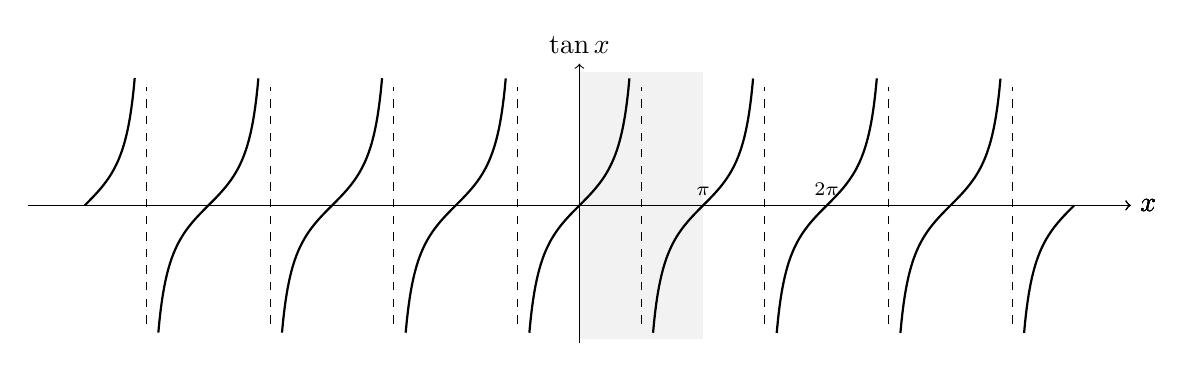
\begin{tikzpicture}[scale=0.5]
\pgfmathsetmacro{\eps}{0.3};
\pgfmathsetmacro{\pisd}{1.5707};
\pgfmathsetmacro{\h}{3};

\pgfmathsetmacro{\Pi}{3.1415};

\fill[color=gray!10] (0,-3.4) rectangle (\Pi,3.4);
\draw [ ->] (0,-3.5)--(0,{3.6}) node[above]{$\tan x$};
\foreach \k in {-2,-1,0,1} {
\draw [ ->] (-14,0)--(14,0) node[right]{$x$};
 \draw [thick, domain={\k*2*\Pi}:{\k*2*\Pi+\pisd-\eps}, samples=100] plot (\x,{(sin(\x
r))/(cos(\x r))});
\draw[dashed] (\k*2*\Pi+\pisd,-\h)--(\k*2*\Pi+\pisd,+\h);
 \draw [thick, domain={\k*2*\Pi+\pisd+\eps}:{\k*2*\Pi+3*\pisd-\eps}, samples=100] plot
(\x,{(sin(\x r))/(cos(\x r))});
\draw[dashed] (\k*2*\Pi+3*\pisd,-\h)--(\k*2*\Pi+3*\pisd,+\h);
 \draw [thick, domain={\k*2*\Pi+3*\pisd+\eps}:{\k*2*\Pi+4*\pisd}, samples=100] plot
(\x,{(sin(\x r))/(cos(\x r))});
}

\draw (\Pi,0) node{$\shortmid$};
\draw (\Pi,0) node[above]{$\scriptstyle{\pi}$};
\draw ({2*\Pi},0) node{$\shortmid$};
\draw ({2*\Pi},0) node[above]{$\scriptstyle{2\pi}$};

\end{tikzpicture}\end{bmlimage}
\end{center}
Observemos que o período da tangente é $\pi$ (e não $2\pi$!), como foi 
visto em \eqref{eqtrigo000}:
$$\boxed{\tan(x+\pi)=\tan x\,,\quad \forall x\in \bR\,.}$$
 
\subsection{Transformações}\index{gráfico! transformação de}
O gráfico de uma função $f$ permite obter os gráficos de outras funções, via
\emph{transformações elementares}.
Para simplificar, nesta seção consideraremos somente funções cujo domínio é a reta toda.
\begin{ex}
Considere o gráfico da função $f(x)=x^2$, a parábola do Exemplo \ref{Ex:Grafxdois}. Qual é a 
função ${g}$ cujo gráfico é o gráfico de $f$ 
\emph{transladado de $3$ unidades para a direita?}
\begin{center}
\begin{bmlimage}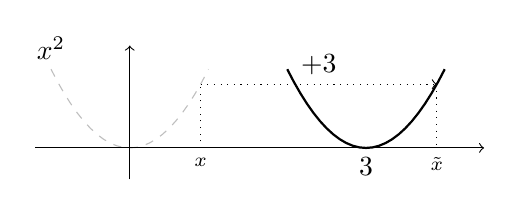
\begin{tikzpicture}
\draw [color=gray!50, dashed, domain=-1:1] plot (\x,{(\x)^2});
\draw (-1,1) node[above]{$x^2$};
\draw [thick, domain=2:4] plot (\x,{(\x-3)^2});
%\draw (2,1) node[above]{$?$};
\draw (3,0) node[below]{$3$};
\draw [ ->] (-1.2,0)--(4.5,0);
\draw [ ->] (0,-0.4)--(0,1.3);
\pgfmathsetmacro{\a}{0.9};
\draw (\a,0) node[below]{$\scriptstyle{x}$};
\draw (3,0) node{$\shortmid$};
\draw (\a+3,0) node[below]{$\scriptstyle{\tilde{x}}$};
\draw[dotted] (\a,0)--(\a,{\a^2});
\draw[dotted, ->] (\a,{\a^2})--(\a+3,{\a^2}) node[midway, above]{$+3$};
\draw[dotted] (\a+3,{\a^2})--(\a+3,0);
\end{tikzpicture}\end{bmlimage}
\end{center}
 Vemos que o valor tomado por ${{g}}$ em $\tilde{x}=x+3$ deve ser o mesmo que o valor tomado por
$f$ em $x$: ${{g}}(\tilde{x})=f(x)$. Como $x=\tilde{x}-3$, ${{g}}(\tilde{x})=f(\tilde{x}-3)$. Logo, a função procurada
é ${{g}}(x)=(x-3)^2$.
\end{ex}

 De modo geral, suponha $f(x)$ definida para todo $x$, e $a\neq 0$ um número fixo. Defina
a função $g$ por
$$g(x)\pardef f(x-a)\,.$$
 Então o gráfico de $g$ é obtido \emph{transladando horizontalmente o gráfico de $f$ de
$a$ unidades.}\index{translação! horizontal} Apesar do sinal ``$-$'', 
a translação é \emph{para a direita se $a>0$, e para a esquerda se $a<0$}.\\

Por outro lado, se $b\in \bR$, 
$$h(x)\pardef f(x)+b\,$$
é uma função cujo gráfico é o gráfico de $f$ \emph{transladado verticalmente de $b$
unidades.}\index{translação! vertical} A translação é \emph{para cima se $b>0$, para baixo
se $b<0$}.

\begin{ex}\label{exemplo_Funcoes_grafparabdesloc}
 Esbocemos o gráfico da função $f(x)=x^2+2x$. Completando o quadrado\index{completar um
quadrado}, $f(x)=(x+1)^2-1$. Portanto, o gráfico de $f$ é obtido a partir da
parábola\index{parábola} $x^2$ pela composição de uma translação horizontal de uma
unidade para a esquerda, e em seguida uma translação vertical de uma unidade para
baixo:
\begin{center}
\begin{bmlimage}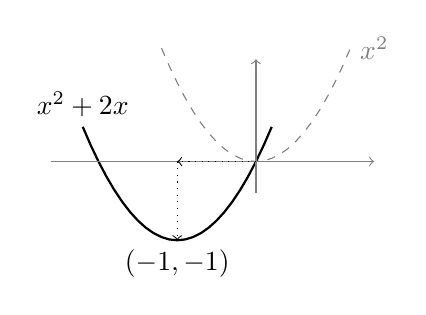
\begin{tikzpicture}
\draw [gray=!30, dashed, domain=-1.2:1.2] plot (\x,{(\x)^2}) node[right]{$x^2$};
%\draw (-1,1) node[above]{$x^2$};
\draw [thick, domain=-2.2:0.2] plot (\x,{(\x+1)^2-1}) ;
\draw (-2.2,{(-2.2+1)^2-1}) node[above]{$x^2+2x$};
%\draw (-1,0) node[above]{$-1$};
\draw (-1,0) node{$\shortmid$};
\draw [gray=!30,  ->] (-2.6,0)--(1.5,0);
\draw [gray=!30,  ->] (0,-0.4)--(0,1.3);
\draw[dotted, ->] (0,0)--(-1,0);
\draw[dotted, ->] (-1,0)--(-1,-1);
\draw (-1,-1) node[below]{$(-1,-1)$};
\end{tikzpicture}\end{bmlimage}
\end{center}
\end{ex}

É claro que o gráfico de $g(x)\pardef -f(x)$ é obtido fazendo a reflexão\index{reflexão}
do gráfico em relação ao eixo $x$, e que o gráfico de $h(x)\pardef f(-x)$ é obtido fazendo
a reflexão do gráfico em relação ao eixo $y$. Portanto, se $f$ é par, $h$ e $f$ têm o
mesmo gráfico. 

\begin{exo}
Considere uma função $f$ definida na reta toda, e a reta vertical $r:$ $x=a$.
Dê a função $g$ cujo gráfico é obtido pelo gráfico de $f$ por \grasA{reflexão em relação à
reta $r$}. Faça a mesma coisa com uma reta horizontal.
\begin{sol}
Se a reta for vertical ($x=a$): $g(x)\pardef f(2a-x)$.
Se a reta for horizontal ($y=b$): $g(x)\pardef 2b-f(x)$.
\end{sol}
\end{exo}

Finalmente, estudemos o que acontece com $g(x)\pardef |f(x)|$. 
Sabemos que o gráfico de $g$ é o mesmo que o de $f$ em todos os pontos $x$ onde $f(x)\geq
0$. Por outro lado, quando $f(x)<0$, então $g(x)=-f(x)$, isto é, o gráfico de $g$ em $x$ é
o de $f$ refletido em relação ao eixo $x$. Em outras palavras: o gráfico 
de $|f|$ é obtido
refletindo todas as partes do gráfico de $f$ negativas, tornando-as 
positivas.
\begin{ex}\label{Ex:modulodografico}
Como $x^2-1$ é a parábola transladada de uma unidade para baixo, o gráfico de $|x^2-1|$ é dado por:
\begin{center}
\begin{bmlimage}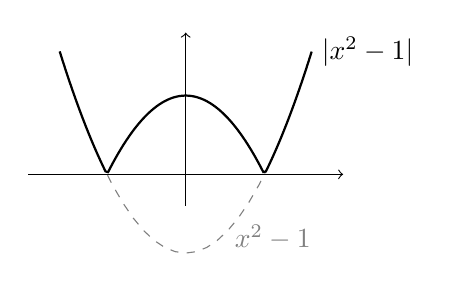
\begin{tikzpicture}
\pgfmathsetmacro{\a}{1.6};
\draw [gray=!30, dashed, domain=-\a:\a] plot (\x,{(\x)^2-1});
\draw [thick, domain=-\a:\a, samples=100] plot (\x,{abs((\x)^2-1)}) node[right]{$|x^2-1|$};
\draw[gray=!30] (0.5,-0.8) node[right]{$x^2-1$};
\draw [ ->] (-2,0)--(2,0);
\draw [ ->] (0,-0.4)--(0,1.8);
\end{tikzpicture}\end{bmlimage}
\end{center}
\end{ex}

\begin{exo}
 Interprete todas as identidades trigonométricas\index{identidades trigonométricas} do
Exercício \ref{exorelattrigo} como tranformações dos gráficos de $\sen$, $\cos$ e $\tan$.
\end{exo}

\begin{exo}\label{Ex:graficosbasicos}
Esboce os gráficos das seguintes funções:
\begin{multicols}{3}
 \begin{enumerate}
  \item $f(x)=1-|\sen x|$
  \item $g(x)=x+1-x^2$
  \item $h(x)=||x|-1|$
\item $i(x)=2\sen x$
\item $j(x)=\half\sen x$
\item $k(x)=\frac{2x-x^2}{(x-1)^2}$
 \end{enumerate}
\end{multicols}
\vspace{0.01cm}
\begin{sol}\mbox{}
\begin{center}
 \begin{bmlimage}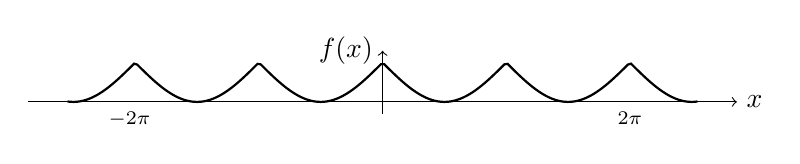
\begin{tikzpicture}[scale=0.5]
\draw [thick, domain=-8:8, samples=200] plot (\x,{1-abs(sin(\x r))});
\draw [ ->] (-9,0)--(9,0) node[right]{$x$};
\draw [ ->] (0,-0.3)--(0,{1.3}) node[left]{$f(x)$};
\pgfmathsetmacro{\Pi}{3.1415};
\draw ({-2*\Pi},0) node[below]{$\scriptstyle{ -2\pi}\,\,\,$};
\draw ({-2*\Pi},0) node{$\shortmid$};
\draw ({2*\Pi},0) node[below]{$\scriptstyle{ 2\pi}$};
\draw ({2*\Pi},0) node{$\shortmid$};
 \end{tikzpicture}\end{bmlimage}
\end{center}
Observe que o período de $f$ é $\pi$. Completando o quadrado\index{completar um quadrado},
$g(x)=-(x-\tfrac12)^2+\tfrac{5}{4}$:
\begin{center}
\begin{bmlimage}\begin{tikzpicture}
\draw [thick, domain=-0.8:1.8] plot (\x,{1.25-(\x-0.5)^2}) ;
\draw[dotted] (0,1.25)--(0.5,1.25)--(0.5,0);
\draw (0.5,1.25) node[above]{$\scriptstyle{(\tfrac12,\tfrac54)}$};
\fill (0.5,1.25) circle (0.45mm);
\draw [ ->] (-1,0)--(1.9,0);
\draw [ ->] (0,-0.4)--(0,1.7) node[left]{$g(x)$};
\end{tikzpicture}\end{bmlimage}
\end{center}
 Observe que a parábola corta o eixo $x$ nos pontos solução da equação $g(x)=0$, que são
$\frac{1\pm \sqrt{5}}{2}$.
 O gráfico da função $h$ já foi esboçado no Exercício \ref{Ex:graficosbasicos}. Mas aqui
vemos que ele pode ser obtido a partir do gráfico de $|x|$ por uma translação de $1$ para
baixo, composta por uma reflexão das partes negativas.
Como $i(x)$ é igual ao dobro de $\sen x$ e $j(x)$ à metade de $\sen x$, temos:
\begin{center}
 \begin{bmlimage}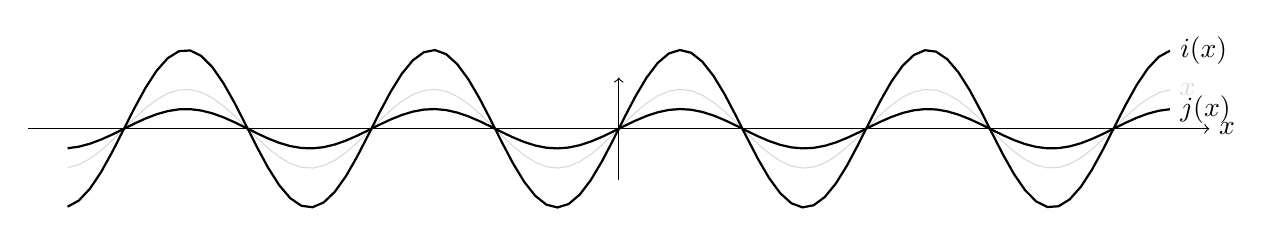
\begin{tikzpicture}[scale=0.5]
 \draw [color=gray!30, domain=-14:14, samples=100] plot (\x,{sin(\x r)})
node[color=gray!30, right]{$\sen x$};
\draw [thick, domain=-14:14, samples=100] plot (\x,{2*sin(\x r)}) node[right]{$i(x)$};
\draw [thick, domain=-14:14, samples=100] plot (\x,{0.5*sin(\x r)}) node[right]{$j(x)$};
\draw [ ->] (-15,0)--(15,0) node[right]{$x$};
\draw [ ->] (0,-1.3)--(0,{1.3});
\pgfmathsetmacro{\Pi}{3.1415};
 \end{tikzpicture}\end{bmlimage}
\end{center}
Completando o quadrado do numerador:
$k(x)=\frac{1-(x-1)^2}{(x-1)^2}=\frac{1}{(x-1)^2}-1$. Portanto, o gráfico pode ser obtido
a partir do gráfico de $\frac{1}{x^2}$:
\begin{center}
\begin{bmlimage}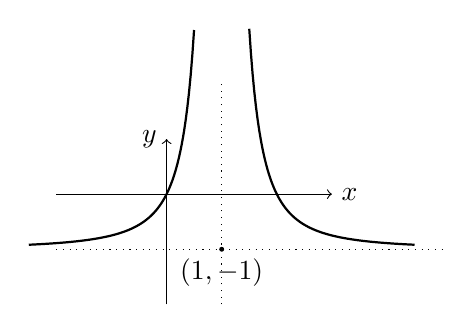
\begin{tikzpicture}[scale=0.7]
\pgfmathsetmacro{\a}{3.5}
\draw [thick, domain=-\a:-0.5, samples=100] plot (\x,{1/((\x)^2)});
\draw [thick, domain=0.5:\a, samples=100] plot (\x,{1/((\x)^2)});
\draw [ ->] (-1,-1)--(-1,2) node[left]{$y$};
\draw [ ->] (-3,1)--(2,1) node[right]{$x$};
\draw[dotted] (-3,0)--(4,0);
\draw[dotted] (0,-1)--(0,3);
\fill (0,0) circle (0.45mm);
\draw (0,0) node[below]{$(1,-1)$};
\end{tikzpicture}\end{bmlimage}
\end{center}
\end{sol}
\end{exo}

\begin{exo}\label{Exo:TrajetPartic}
Uma partícula de massa $m$ 
é lançada da origem com uma velocidade $\vec{v}=\binom{v_{\textsf{h}}}{v_{\textsf{v}}}$. 
A resolução da segunda equação de Newton mostra que a sua trajetória é dada pela função 
$$x\mapsto y(x)=-\frac12 g\Big(
\frac{x}{v_{\textsf{h}}}\Big)^2+\frac{v_\textsf{v}}{v_{\textsf{h}}}x\,,$$
onde $g$ é o campo de gravitação.
Descreva essa trajetória. Em particular, calcule 
 1) a qual distância a partícula vai cair no chão, e compare essa distância quando $g$ é a
constante de gravitação na superfície da terra ($g=9.81m/s^2$), ou na superfície da lua
($g=1.63m/s^2$, seis vezes menor do que na terra), 2) as coordenadas $(x_*,y_*)$ do ponto
mais alto da trajetória.
\begin{sol}
A trajetória é uma \emph{parábola}.
Resolvendo $y(x)=0$ para $x$, obtemos os pontos onde a parábola toca o chão: $x_1=0$
(ponto de partida), e 
$x_2=\frac{2v_{\textsf{v}}v_{\textsf{h}}}{g}$ (distância na qual a partícula vai cair no
chão).
É claro que se o campo de gravitação é mais fraco (na lua por exemplo), $g$ é menor, logo
$x_2$ é maior: o objeto vai mais longe.
Por simetria sabemos que a abcissa do ponto mais alto da trajetória é 
$x_*=\frac{x_2}{2}=\frac{v_{\textsf{v}}v_{\textsf{h}}}{g}$, e a sua abcissa é dada por
$y_*=y(x_*)=\tfrac12 \frac{v_{\textsf{v}}^2}{g}$. Observe que $y_*$ \emph{não depende de
$v_{\textsf{h}}$}.
O ponto $(x_*,y_*)$ pode também ser calculado a partir da trajetória $y(x)$, completando
o quadrado.
\end{sol}
\end{exo}

Um gráfico permite (em princípio) resolver uma inequação graficamente\index{inequação!
resolução gráfica}. 
\begin{ex}
Considere a inequação do Exemplo \ref{Ex:inequmodulo} (último capítulo),
$$|x-2|>3\,.$$
Com $f(x)=|x-2|$ e $g(x)=3$, o conjunto das soluções da inequação, $S$, pode ser
interpretado como o conjunto dos pontos onde o gráfico de $f$ fica
\emph{estritamente acima} do gráfico de $g$: $f(x)>g(x)$. Como o gráfico de $g$
é uma reta horizontal e 
o de $f$ é o gráfico de $|x|$ transladado de duas unidades para a direita,
\begin{center}
\begin{bmlimage}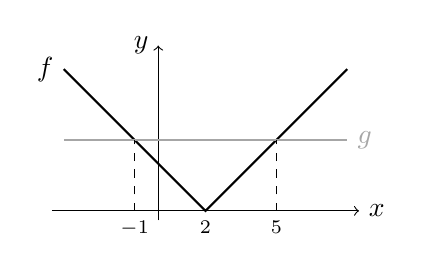
\begin{tikzpicture}[scale=0.3]
\draw [ ->] (-4.5,0)--(8.5,0) node[right]{$x$};
\draw [ ->] (0,-0.4)--(0,7) node[left]{$y$};
\draw[thick] (8,6)--(2,0)--(-4,6) node[left]{$f$};
\draw[color=gray!70, thick] (-4,3)--(8,3) node[right]{$g$};
\pgfmathsetmacro{\x}{-1};
\pgfmathsetmacro{\y}{abs(\x-2)};
\draw (\x,0) node{$\shortmid$};
\draw (\x,0) node[below]{$\scriptstyle{-1}$};
\draw[dashed] (\x,0)--(\x,\y);
\draw (2,0) node{$\shortmid$};
\draw (2,0) node[below]{$\scriptstyle{2}$};
\pgfmathsetmacro{\x}{5};
\pgfmathsetmacro{\y}{abs(\x-2)};
\draw (\x,0) node{$\shortmid$};
\draw (\x,0) node[below]{$\scriptstyle{5}$};
\draw[dashed] (\x,0)--(\x,\y);
\end{tikzpicture}\end{bmlimage}
\end{center}
vemos que todos os pontos em $(-\infty,-1)\cup (5,\infty)$ satisfazem a essa condição, que
é o que tinha sido encontrado anteriormente.
\end{ex}

\begin{exo}
 Resolva graficamente: 
\begin{multicols}{3}
\begin{enumerate}
\item\label{itineqgraf1}  $1-|x-1|\geq |x|$
\item\label{itineqgraf2}  $1-|x-1|> |x|$
\item\label{itineqgraf3}  $|x^2-1|<1$
\end{enumerate}
\end{multicols}
\vspace{0.01cm}
\begin{sol} \eqref{itineqgraf1} Se $f(x)=1-|x-1|$, $g(x)=|x|$,
\begin{center}
\begin{bmlimage}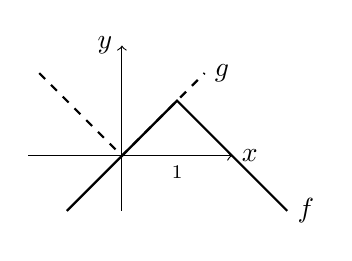
\begin{tikzpicture}[scale=0.7]
\draw [ ->] (-1.7,0)--(2,0) node[right]{$x$};
\draw [ ->] (0,-1)--(0,2) node[left]{$y$};
\draw[thick, dashed] (-1.5,1.5)--(0,0)--(1.5,1.5) node[right]{$g$};
\draw[thick] (-1,-1)--(1,1)--(3,-1) node[right]{$f$};
\pgfmathsetmacro{\x}{-1};
\pgfmathsetmacro{\y}{abs(\x-2)};
\draw (1,0) node{$\shortmid$};
\draw (1,0) node[below]{$\scriptstyle{1}$};
\end{tikzpicture}\end{bmlimage}
\end{center}
Logo, $S=[0,1]$. Para \eqref{itineqgraf2}, $S=\varnothing$.
\eqref{itineqgraf3} Se $f(x)=|x^2-1|$ (veja o gráfico do Exemplo
\ref{Ex:modulodografico}), vemos que $S=(-\sqrt{2},0)\cup(0,\sqrt{2})$.
\end{sol}
\end{exo}

\section{Montar funções}\index{montar funções}

Será sempre necessário, no estudo de certos problemas, \emph{montar} uma função que
satisfaça a algumas condições.

\begin{exo}
 Uma esfera\index{esfera} é pintada com uma tinta cujo custo é de $\mathrm{R}\$10,00$ por
metro quadrado. 
Expresse o custo total da tinta necessária em função do raio (medido em metros) da
esfera, $T(r)$.
Em seguida, a esfera é enchida de concreto, a $\mathrm{R}\$30,00$ o metro cúbico. Expresse
o 
custo total de concreto necessário em função da superfície (medida em metros quadrados)
da esfera, $C(s)$.
\begin{sol}
Tinta: Como a esfera tem superfície igual a $4\pi r^2$, temos $T(r)=40\pi r^2$ 
(onde $r$ é medido em metros).
Concreto: Como o volume é dado por $V=\tfrac43\pi r^3$, o custo de concreto em 
função do raio é $C(r)=40\pi r^3$. Como a superfície $s=4\pi r^2$ temos 
$r=\sqrt{s/4\pi}$. Portanto, 
$C(s)=40\pi(\tfrac{s}{4\pi})^{3/2}$.
\end{sol}
\end{exo}

\begin{exo}
 Considere um ponto $P=(a,b)$ na reta $2y+x=2$.
Expresse $d(a)$ (respectivamente $d(b)$), 
a distância de $P$ ao ponto $Q=(1,-2)$ em função de $a$ (respectivamente $b$).
\begin{sol}
 Por definição, $d(P,Q)=\sqrt{(a-1)^2+(b+2)^2}$.
Como $2a+b=2$, temos $d(a)=\sqrt{\tfrac54a^2-5a+10}$, e $d(b)=\sqrt{5b^2+5}$.
\end{sol}
\end{exo}

\begin{exo}
Um polígono regular (isto é, com todos os seus lados iguais) com $n$ lados é inscrito em um
disco de raio $r$. Calcule o seu perímetro e a sua área em função de $n$ e $r$.
\begin{sol}
Perímetro: $P(n,r)=2nr\sen (\tfrac{\pi}{n})$.
Área: $A(n,r)=\tfrac12 nr^2\sen(\tfrac{2\pi}{n})$.
\end{sol}
\end{exo}

\begin{exo}
Um recipiente cônico\index{cone} é criado girando o gráfico da função $|x|$ em torno do
eixo $y$.
 O objetivo é usar esse recipiente para criar um medidor de volumes (digamos, em metros
cúbicos). Explique como que a marcação do eixo $y$ deve ser feita: $1m^3$, $2m^3$, ...
Faça um esboço desse medidor.
\begin{sol}
Suponha que o cone fique cheio de água, até uma altura de $h$ metros. Isso representa um
volume de 
$V(h)=\tfrac13 (\pi h^2)\times h$ metros cúbicos. Logo, $h(V)=(\tfrac{3 V}{\pi})^{1/3}$.
Assim, a marca para $1m^3$ deve ficar na altura $h(1)\simeq 0.98$, para $2$ metros
cúbicos, $h(2)\simeq 1.24$, etc.
\begin{center}
\begin{bmlimage}\begin{tikzpicture}
 \draw (-3,3)--(0,0)--(3,3)--cycle;
 \fill[areagrafico] (-3,3)--(0,0)--(3,3)--cycle;
\draw (0,0)--(0,3);
\foreach \k in {1,...,5}{
\pgfmathsetmacro{\h}{(((3*\k)/3.141)^(0.333333))};
\draw (0,{\h}) node{$-$};
\draw[dotted] ({-\h},\h)--(\h,\h) node[right]{$\scriptscriptstyle{\k m^3}$};
}
\foreach \k in {6,...,28}{
\pgfmathsetmacro{\h}{(3*\k/3.1414)^(0.333333)};
\draw (0,{\h}) node{$-$};
\draw[dotted] ({-\h},{\h})--({\h},{\h});
}
\end{tikzpicture}\end{bmlimage}
\end{center}

\end{sol}
\end{exo}

\begin{exo}
Uma corda\index{corda} de tamanho $L$ é cortada em dois pedaços. Com o primeiro pedaço,
faz-se um quadrado, e com o segundo, um círculo. Dê a área total (quadrado $+$ círculo) em
função do tamanho do primeiro pedaço. Dê o domínio dessa função.
\begin{sol}
Seja $x$ o tamanho do primeiro pedaço. Como os lados do quadrado medem
$\tfrac{x}{4}$, a área do quadrado é $\tfrac{x^2}{16}$. O círculo tem
circunferência igual a $L-x$, logo o seu raio vale $\tfrac{L-x}{2\pi}$, e a sua
área 
$\pi(\tfrac{L-x}{2\pi})^2=\tfrac{(L-x)^2}{4\pi}$. Portanto a área total é dada por
$A(x)=\tfrac{x^2}{4}+\tfrac{(L-x)^2}{4\pi}$, e o seu domínio é $D=[0,L]$.
\end{sol}
\end{exo}

\begin{exo}\label{Exo:airesousladroite}
Um triângulo $ABC$ é isósceles em $A$, com $|AB|=|AC|=1$.
Dê a área do triângulo em função do ângulo entre $AB$ e $AC$.
Em seguida, esboce essa função no seu domínio, e ache o ângulo para o qual a área é máxima.
\begin{sol}
Seja $\alpha$ o ângulo entre $AB$ e $AC$.
Área: $A(\alpha)=\sen \tfrac{\alpha}{2}\cos\tfrac{\alpha}{2}=\tfrac12\sen \alpha$, com
$D=(0,\pi)$. 
Logo, (olhe para a função $\sen \alpha$), a área é máxima para $\alpha=\tfrac{\pi}{2}$.
\end{sol}
\end{exo}

\begin{exo}\label{Exo:primeiraarea}
 Considere a reta $r:\, y=x+1$, e os pontos $P=(1,0)$, $Q=(t,0)$, $t>1$. 
Seja $R_t$ a região delimitada pela reta $r$, pelo eixo $x$, 
e pelas retas verticais passando por $P$ e $Q$. Esboce $R_t$, e expresse a sua área
$A(t)$ em  função de $t$.
\begin{sol}
A área pode ser calculada via uma diferença de dois triângulos:
\begin{center}
\begin{bmlimage}\begin{tikzpicture}
\fill[areagrafico] (1,0)--(1,2)--plot[domain=1:2.5](\x,{\x+1})--(2.5,0)--cycle;
\draw[dotted] (1,0)--(1,2);
\draw (1,0) node{$\shortmid$};
\draw (1,0) node[below]{$1$};
\draw[dotted] (2.5,0)--(2.5,3.5);
\draw (2.5,0) node{$\shortmid$};
\draw (2.5,0) node[below]{$t$};
\draw (2.5,-0.1) node[below left]{$\leftarrow$};
\draw (2.5,-0.1) node[below right]{$\rightarrow$};
\draw [ ->] (0,-0.2)--(0,3);
\draw [ ->] (-0.2,0)--(3.5,0);
\draw[thick] (-0.5,0.5)--(3,4) node[right]{$r:\,y=x+1$};
\draw (5,2) node[right]{$A(t)=\tfrac{t^2}{2}+t-\tfrac32$};
\draw (1.7,1.3) node{$R_t$};
\end{tikzpicture}\end{bmlimage}
\end{center}
%\caption{Truc}
%\end{figure}
\end{sol}
\end{exo}


\begin{exo}

Considere uma pirâmide\index{pirâmide} $\Pi$ de altura $H$, cuja base é um quadrado de
lado $L$ ($H$ e $L$ são constantes). Considere em seguida a pirâmide truncada $\Pi'$
obtida cortando $\Pi$ horizontalmente, na altura de um ponto 
$P$ na aresta lateral, como na ilustração. 
\begin{center}
\begin{bmlimage}\begin{tikzpicture}[scale=1.5]
\pgfmathsetmacro{\L}{1};
\pgfmathsetmacro{\H}{2};
\coordinate (A) at (\L,0,\L);
\coordinate (B) at (\L,0,-\L);
\coordinate (C) at (-\L,0,-\L);
\coordinate (D) at (-\L,0,\L);
\coordinate (S) at (0,\H,0);
\coordinate (P) at ({\L/2},{\H/2},{-\L/2});
\coordinate (Q) at ({\L/2},{\H/2},{\L/2});
\coordinate (R) at ({-\L/2},{\H/2},{\L/2});
\coordinate (T) at ({-\L/2},{\H/2},{-\L/2});

\draw[thin] (S)--(D)--(C)--cycle;
\draw[thin] (S)--(C)--(B)--cycle;
\draw (S) node[left]{$S$};
\fill[areagrafico, opacity=0.5] (P)--(B)--(A)--(Q)--cycle;
\draw (B) node[right]{$B$};
\fill[areagrafico, opacity=0.5] (P)--(Q)--(R)--(T)--cycle;
\draw (P) node[above right]{$P$};
\fill[areagrafico, opacity=0.5] (Q)--(R)--(D)--(A)--cycle;
\draw[thick] (P)--(Q)--(R)--(T)--cycle;
\draw[thick] (P)--(B)--(A)--(Q)--cycle;
\draw[thick] (Q)--(R)--(D)--(A)--cycle;
\draw[thin] (S)--(D)--(A)--cycle;
\draw[thin] (S)--(A)--(B)--cycle;
\fill (P) circle (0.5mm);
\end{tikzpicture}\end{bmlimage}
\end{center}
Expresse o volume e a área da superfície de $\Pi'$ em função da distância $x=|PB|$.
\end{exo}

\section{Composição, contradomínio e imagem}

Suponha que se queira obter o valor de $\sen (\pi^2)$ com uma
calculadora. Como uma calculadora possui em geral as duas funções
$(\cdot)^2$ e $\sen(\cdot)$, calculemos primeiro o quadrado de $\pi$, e
em seguida tomemos o seno do resultado:
\[
\pi=3.1415...\stackrel{(\cdot)^2}{\longmapsto} \pi^2=9,8696...
\stackrel{\sen(\cdot)}{\longmapsto} 
\sen(\pi^2)=-0.4303...
\]
O que foi feito foi \emph{compor} duas funções.\\

Sejam $f$ e $g$ duas funções reais. Definemos a \grasA{composição de $f$ com
$g$}\index{função! composição de } como a nova função $f\circ g$ definida por
$$\boxed{(f\circ g)(x)\pardef f(g(x))\,.}$$
Isto significa que para calcular $x\mapsto (f\circ g)(x))$, 
calculamos \emph{primeiro} $g(x)$,
$$x\mapsto g(x)\,,$$
e \emph{em seguida} aplicamos $f$:
$$x\mapsto g(x)\mapsto f(g(x))\,.$$

\begin{exo}
Sejam $f(x)=x^2$, $g(x)=\frac{1}{x+1}$, $h(x)=x+1$. Calcule 
$$(f\circ g)(0)\,, (g\circ f)(0)\,, (f\circ g)(1)\,, (g\circ f)(1)\,, f(g(h(-1)))\,,
h(f(g(3)))\,.$$
\begin{sol} Como $f(g(x))=\frac{1}{(x+1)^2}$, $g(f(x))=\frac{1}{x^2+1}$, temos
$(f\circ g)(0)=1$, $(g\circ f)(0)=1$, $(f\circ g)(1)=\frac14$, $(g\circ f)(1)=\frac12$.
Como $f(g(h(x)))=\frac{1}{(x+2)^2}$ e $h(f(g(x)))=\frac{1}{(x+1)^2}+1$, 
 $f(g(h(-1)))=1$,
$h(f(g(3)))=\frac{17}{16}$.
\end{sol}
\end{exo}

Como foi observado no exercício anterior, $f\circ g$ é em geral diferente de $g\circ f$.\\

Às vezes será necessário considerar uma função complicada como sendo uma composta de
funções mais elementares:
\begin{ex}
A função $x\mapsto \sqrt{1+x^2}$ pode ser vista como a composta
$$x\mapsto 1+x^2\mapsto\sqrt{1+x^2}\,,$$
que significa que $\sqrt{1+x^2}=f(g(x))$, com $g(x)=1+x^2$ e $f(x)=\sqrt{x}$.
Observe que podia também escrever 
$$x\mapsto x^2\mapsto 1+x^2\mapsto \sqrt{1+x^2}\,,$$
que dá a decomposição $\sqrt{1+x^2}=f(g(h(x)))$, onde $h(x)=x^2$, $g(x)=x+1$,
$f(x)=\sqrt{x}$.
\end{ex}

\begin{exo}\label{Exo_elem_decomp_compos}
Para cada função $f$ a seguir, dê uma decomposição de $f$ como composição de funções mais
simples. 
\begin{multicols}{3}
\begin{enumerate}
\item\label{itexcompos1} $\sen (2x)$
\item\label{itexcompos2} $\frac{1}{\sen x}$
\item\label{itexcompos3} $\sen (\tfrac1x)$
\item\label{itexcompos4} $\sqrt{\frac{1}{\tan (x)}}$
\end{enumerate}
\end{multicols}
\vspace{0.01cm}
\begin{sol}
\eqref{itexcompos1} $\sen (2x)=f(g(x))$, onde $g(x)=2x$, $f(x)=\sen x$.
\eqref{itexcompos2} $\frac{1}{\sen x}=f(g(x))$, onde $g(x)=\sen x$, $f(x)=\frac1x$.
\eqref{itexcompos3} $\sen(\frac{1}{x})=f(g(x))$, onde $f(x)=\sen x$, $g(x)=\frac1x$.
\eqref{itexcompos4} $\sqrt{\frac{1}{\tan (x)}}=f(g(h(x)))$, onde $f(x)=\sqrt{x}$,
$g(x)=\frac{1}{x}$, $h(x)=\tan x$.
\end{sol}

\end{exo}

\begin{exo}
Considere
$$
f(x)\pardef 
\begin{cases}
 x+3&\text{ se }x\geq 0\,,\\
x^2&\text{ se }x<0\,,
\end{cases}
\quad\quad
g(x)\pardef 
\begin{cases}
 2x+1&\text{ se }x\geq 3\,,\\
x&\text{ se }x<3\,.
\end{cases}
$$
Calcule $f\circ g$ e $g\circ f$.
\begin{sol}
$$
(g\circ f)(x)=
\begin{cases}
 2x+7&\text{ se }x\geq 0\,,\\
x^2&\text{ se }-\sqrt{3}<x<0\,,\\
2x^2+1&\text{ se }x\leq -\sqrt{3}\,.
\end{cases}
\quad\quad
(f\circ g)(x)=
\begin{cases}
 2x+4&\text{ se }x\geq 3\,,\\
x+3&\text{ se }0\leq x<3\,,\\
x^2&\text{ se }x<0\,.
\end{cases}
$$
\end{sol}
\end{exo}

Lembramos que uma função é sempre definida junto com o seu domínio:
\begin{align*}
f:D&\to \bR\\
x&\mapsto f(x)\,.
\end{align*}
Em ``$f:D\to \bR$'', o ``$\bR$'' foi colocado para indicar que qualquer 
que seja $x$,
$f(x)$ é sempre um número real. Em outras palavas: a imagem de qualquer 
$x\in D$ por $f$ é um número real.
Vejamos em alguns exemplos que esse conjunto ``$\bR$'' pode ser mudado 
por um conjunto que represente melhor a função.

\begin{ex}
Considere
\begin{align*}
f:\bR&\to \bR\\
x&\mapsto x^2\,.
\end{align*}
Como $x^2\geq  0$ qualquer que seja $x\in \bR$, 
vemos que a imagem de qualquer $x\in \bR$ por $f$ é positiva.
Logo, podemos rescrever a função da seguinte maneira:
\begin{align*}
f:\bR&\to [0,\infty)\\
x&\mapsto x^2\,.
\end{align*}
\end{ex}

Quando uma função for escrita na forma 
\begin{align*}
f:D&\to C\\
x&\mapsto f(x)\,,
\end{align*}
para indicar que qualquer $x$ em $D$ tem a sua imagem em $C$, diremos que um
\grasA{contradomínio} foi escolhido para $f$. Em geral, não existe uma escolha única para
o contradomínio.

\begin{ex}
Como, $x\mapsto \sen x$ é uma função limitada, podemos escrever 
\begin{align}
\sen:\bR&\to [-10,+10]\label{eq:contradomsen}\\
x&\mapsto \sen x\,.\nonumber
\end{align}
Mas podemos também escolher um contradomínio menor:
\begin{align}
\sen:\bR&\to [-1,+1]\label{eq:contradomsen}\\
x&\mapsto \sen x\,.\nonumber
\end{align}
Acontece que $[-1,+1]$ é o menor contradomínio possível (ver abaixo).
\end{ex}

% \begin{ex} Para voltar à discussão anterior, considere
% $f(x)=\sqrt{x}$ e $g(x)={1-x}$. Para $(f\circ g)(x)=f(g(x))$ ser bem definida, vemos 
% $x$ precisa ser tal que
% $g(x)1-x\geq 0$. Em outras
% Isto é, $x\in (-\infty,1]$. 
% \end{ex}

 Seja $f:D\to C$. Para cada $x\in D$, lembremos que $f(x)\in C$ é chamado de \emph{imagem
de $x$}\index{imagem}, e o
\grasA{conjunto imagem} de $f$ é definido como
$$\boxed{\imagem(f)\pardef \{f(x):x\in D\}\,.}$$
Por definição, $\imagem(f)\subset C$ é um contradomínio, e é também o menor possível.
Para cada $y\in \imagem(f)$, existe pelo menos um $x\in D$ tal que $f(x)=y$, cada $x$ com
essa propriedade é chamado de \grasA{preimagem}\index{preimagem} de $y$. 
 Cada ponto $x\in D$ possui uma única imagem em $C$, um $y\in C$ pode possuir uma
preimagem, mais de uma preimagem, ou nenhuma preimagem.

\begin{ex}
Considere a função seno na reta.
 Ao $x$ percorrer a reta real, $\sen x$ atinge todos os pontos do intervalo $[-1,1]$. Logo,
$\imagem(\sen)=[-1,1]$. Qualquer $y\in [-1,1]$ possui infinitas preimagens, por exemplo,
todos os pontos de $\{k\pi,k\in \bZ\}$ são preimagens de 
 $y=0$. O ponto $y=2$, por sua vez, não possui nenhuma preimagem (não existe $x\in \bR$
tal que $\sen x=2$).
\end{ex}

\begin{exo} Calcule o conjunto imagem das seguintes funções: 
\begin{multicols}{3}
\begin{enumerate}
\item\label{itconjimagem1} $-2x+1$, $D=\bR$
\item\label{itconjimagem2} $-2x+1$, $D=[-1,1]$
\item\label{itconjimagem21} $x^p$ ($p$ ímpar) 
\item\label{itconjimagem22} $x^p$ ($p$ par)
\item\label{itconjimagem3} $\tfrac{1}{x}$, $D=\bR\setminus \{0\}$
\item\label{itconjimagem4} $\tfrac{1}{x}$, $D=(0,\infty)$
\item\label{itconjimagem5a} $x^2+1$, $D=\bR$
\item\label{itconjimagem5} $1-x^2$, $D=\bR$
\item\label{itconjimagem51} $x^2+2x$, $D=(-\infty,0)$
\item\label{itconjimagem6} $\tan x$,
\item\label{itconjimagem7} $\sen x$, $D=[-\pisobredois,\pisobredois]$
\item\label{itconjimagem8} $\cos x$, $D=(-\pisobredois,\pisobredois)$
\item\label{itconjimagem801} $\tfrac13\sen x$, $D=\bR$
\item\label{itconjimagem81} $\sen (\pisobrequatro\sen x)$, $D=\bR$
\item\label{itconjimagem9} $\frac{1}{x^2+1}$, $D=\bR$ 
\item\label{itconjimagem10} $\begin{cases}x+1&\text{ se }x\geq0\\\tfrac12(x-1)&\text{ se } x<0\end{cases}$
\end{enumerate}
\end{multicols}
\vspace{0.01cm}
Faça a mesma coisa com as funções do Exercício \eqref{ExoEsbocosElementares}.
\begin{sol}
\eqref{itconjimagem1} $\imagem(f)=\bR$,
\eqref{itconjimagem2} $\imagem(f)=[-1,3]$,
\eqref{itconjimagem21} Se $p>0$ então $D=\bR$ e $\imagem(f)=\bR$. Se 
$p<0$ então $D=\bR\setminus\{0\}$ e $\imagem(f)=\bR\setminus\{0\}$
\eqref{itconjimagem22} $\imagem(f)=[0,\infty)$ se $p>0$, $\imagem(f)=(0,\infty)$ se $p<0$,
\eqref{itconjimagem3} $\imagem(f)=\bR\setminus \{0\}$,
\eqref{itconjimagem4} $\imagem(f)=(0,\infty)$,
\eqref{itconjimagem5a} $\imagem(f)=[1,\infty)$,
\eqref{itconjimagem5} $\imagem(f)=(-\infty,1]$,
\eqref{itconjimagem51} $\imagem(f)=[-1,\infty)$,
\eqref{itconjimagem6} $\imagem(f)=\bR$,
\eqref{itconjimagem7} $\imagem(f)=[-1,1]$,
\eqref{itconjimagem8} $\imagem(f)=(0,1]$,
\eqref{itconjimagem801} $\imagem(f)=[-\tfrac13,\tfrac13]$,
\eqref{itconjimagem81} $\imagem(f)=[-\tfrac{1}{\sqrt{2}},\tfrac{1}{\sqrt{2}}]$,
\eqref{itconjimagem9} $\imagem(f)=(0,1]$. De fato, $0<\frac{1}{1+x^2}\leq 1$. Melhor:
se $y\in (0,1]$ então $y=\frac{1}{1+x^2}$ possui uma única solução, dada por
$x=\sqrt{\frac{1-y}{y}}$.
\eqref{itconjimagem10} $\imagem(f)=(-\infty,-\tfrac12)\cup [1,\infty)$.

Para as funções do Exercício \ref{ExoEsbocosElementares}:
$\imagem(f)=(0,\infty)$,
$\imagem(g)=(-\infty,0]$,
$\imagem(h)=\bZ$,
$\imagem(i)=[0,1)$,
$\imagem(j)=[0,\infty)$.
\end{sol}
\end{exo}

\begin{exo}
Se $f(x)=\frac{2x}{x^2+25}$, calcule $\imagem(f)$. Para cada $y\in \imagem(f)$, determine
se $y$ possui uma única preimagem ou mais.
\begin{sol}
Se trata de achar todos os $y\in \bR$ para os quais existe pelo menos um $x\in
\bR$ tal que $f(x)=y$. Isso corresponde a resolver a equação do segundo grau em
$x$: $yx^2-2x+25y=0$. Se $y=0$, então $x=0$. Se $y\neq 0$,
$x=\frac{1\pm\sqrt{1-25y^2}}{y}$, que tem solução se e somente se
$|y|\leq\tfrac15$.
Logo, $\imagem(f)=[-\tfrac15,\tfrac15]$. O ponto $y=0$ é o único que possui uma única preimagem, qualquer outro ponto de $\imagem(f)$ possui duas preimagens. Isso pode ser verificado no gráfico:
\begin{center}
 \begin{bmlimage}\begin{tikzpicture}[scale=0.5]
\draw[->] (-13,0)--(13,0);
\draw[->] (0,-3)--(0,3);
\draw[thick, domain=-12.5:12.5, samples=100] plot (\x,{(60*\x)/(9*(\x)^2+25)});
\draw[dotted] (0,2)node[left]{$\tfrac15$}--(5/3,2);
\draw[dotted] (0,-2)node[right]{$\tfrac15$}--(-5/3,-2);
\draw[dotted,->] (0,1)node[left]{$y$}--(0.5,1)--(0.5,0);
\draw (0,1) node{$-$};
\draw[dotted,->] (0,1)--(0.5,1)--(0.5,0);
\draw[dotted,->] (0,1)--(0.5,1)--(0.5,0);
\draw[dotted,->] (0,1)--(6,1)--(6,0);
 \end{tikzpicture}\end{bmlimage}
\end{center}
\end{sol}
\end{exo}

\subsection{Bijeção, função inversa}

Diremos que uma função $f:D\to C$ é \grasA{bijetiva}\index{função! bijetiva} (ou
simplesmente: $f$ é uma \grasA{bijeção}) 
se
\begin{enumerate} 
\item $\imagem(f)=C$ (isto é, se $f$ atinge cada
ponto do seu contradomínio), e se 
\item 
qualquer $y\in C$ possui uma única preimagem, i.e.
existe um único $x\in D$ tal que
\eq{\label{eq:definverse}f(x)=y\,.} 
\end{enumerate}

Quando uma função é bijetiva, é possivel definir a sua \grasA{função
inversa}\index{função! inversa},
$f^{-1}:C\to D$, onde para todo $y\in C$, $f^{-1}(y)$ é definido como a única
solução $x$ de \eqref{eq:definverse}. A função inversa tem as seguintes
propriedades:
$$\boxed{\forall x\in D, 
\,(f^{-1}\circ f)(x)=x\,, \quad \text{ e } \forall y\in C,\, (f\circ
f^{-1})(y)=y\,.}$$
\begin{ex}\label{exemploinversao}
Considere a função do Exemplo \ref{Ex:retaegrafico}: $f(x)=\tfrac{x}{2}+1$ com $D=[0,2)$.
Então $\imagem(f)=[1,2)$, e $f:[0,2)\to [1,2)$ é uma bijeção:
\begin{center}
\begin{bmlimage}\begin{tikzpicture}
\begin{scope}
\draw [ ->] (0,-0.1)--(0,2.5) node[left]{$y$};
\draw [ ->] (-0.3,0)--(2.5,0) node[right]{$x$};
\draw [thick] (0,1)--(2,2);
\fill[intaberto] (2,2) circle (0.45mm);
%%
\draw[dotted] (0,2)--(2,2);
\draw (0,2) node[left]{$2$};
\draw (0,1) node[left]{$1$};
\draw (0,2) node{$-$};
\draw (0,1) node{$-$};
%%
\draw (0,0) node{$\shortmid$};
\fill (0,1) circle (0.45mm);
\pgfmathsetmacro{\x}{0.8};
\draw (\x,0) node{$\shortmid$};
\draw (\x,0) node[below]{$\scriptstyle{x}$};
\draw[dashed, ->] (\x,0)--(\x,{1+\x/2})--(0,{1+\x/2}) node[left]{$\scriptstyle{f(x)}$};
\draw (0,0) node[below]{$0$};
\draw (2,0) node[below]{$2$};
\draw[dotted] (2,0)--(2,2);
\end{scope}

\begin{scope}[xshift=7cm]
\draw [ ->] (0,-0.1)--(0,2.5) node[left]{$y$};
\draw [ ->] (-0.3,0)--(2.5,0) node[right]{$x$};
\draw [thick] (0,1)--(2,2);
\draw (0,0) node{$\shortmid$};
\fill (0,1) circle (0.45mm);
\fill[intaberto] (2,2) circle (0.45mm);
%%
\draw[dotted] (0,2)--(2,2);
\draw (0,2) node[left]{$2$};
\draw (0,1) node[left]{$1$};
\draw (0,2) node{$-$};
\draw (0,1) node{$-$};
%%
\pgfmathsetmacro{\x}{0.8};
\draw (\x,0) node{$\shortmid$};
\draw (\x,0) node[below]{$\scriptstyle{f^{-1}(y)}$};
\draw[dashed, color=gray!60, <-] (\x,0)--(\x,{1+\x/2})--(0,{1+\x/2}) node[left]{$\scriptstyle{y}$};
\draw (0,0) node[below]{$0$};
\draw (2,0) node[below]{$2$};
\draw[dotted] (2,0)--(2,2);
\end{scope}
\end{tikzpicture}\end{bmlimage}
\end{center}
Como $y=\tfrac{x}{2}+1$, a função inversa obtém-se isolando $x$: $x=2(y-1)$. Logo, 
$f^{-1}:[1,2)\to[0,2)$, 
$f^{-1}(y)=2(y-1)$. 
Para esboçar o gráfico da função inversa no plano cartesiano, é mais natural
\emph{renomear} a variável usada para representar $f^{-1}$, da seguinte maneira:
\begin{align*}
 f^{-1}:[1,2)&\to[0,2)\\
x&\mapsto 2(x-1)\,.
\end{align*}
Podemos agora esbocar $f^{-1}$:
\begin{center}
\begin{bmlimage}\begin{tikzpicture}
\draw [ ->] (0,-0.1)--(0,2.5);
\draw [ ->] (-0.3,0)--(2.5,0) node[right]{$x$};
%\draw [color=gray!30, ->] (0,1)--(2,2);
\draw [thick] (1,0)--(2,2);
\fill[intaberto] (2,2) circle (0.45mm);
%%
\draw[dotted] (0,2)--(2,2);
\draw (0,2) node[left]{$2$};
\draw (1,0) node[below]{$1$};
%\draw (0,2) node{$-$};
\draw (1,0) node{$\shortmid$};
%%
\draw (0,0) node{$\shortmid$};
\fill (1,0) circle (0.45mm);
\pgfmathsetmacro{\x}{1.4};
\draw (\x,0) node{$\shortmid$};
\draw (\x,0) node[below]{$\scriptstyle{x}$};
\draw[dashed, ->] (\x,0)--(\x,{2*(\x-1)})--(0,{2*(\x-1)}) node[left]{$\scriptstyle{f^{-1}(x)}$};
\draw (0,0) node[below]{$0$};
\draw (2,0) node[below]{$2$};
\draw[dotted] (2,0)--(2,2);
\end{tikzpicture}\end{bmlimage}
\end{center}
É importante observar que o gráfico da função inversa obtém-se a partir do
gráfico de $f$ por uma \emph{simetria através da diagonal do primeiro quadrante}:
\begin{center}
\begin{bmlimage}\begin{tikzpicture}
\draw [ ->] (0,-0.1)--(0,2.5);
\draw [ ->] (-0.3,0)--(2.5,0);
\draw [color=gray!30, ->] (0,1)--(2,2);
\draw [thick] (1,0)--(2,2);
\fill[intaberto] (2,2) circle (0.45mm);
%%
\draw[dotted] (0,2)--(2,2);
\draw (0,2) node[left]{$2$};
\draw (1,0) node[below]{$1$};
%\draw (0,2) node{$-$};
\draw (1,0) node{$\shortmid$};
%%
\draw (0,0) node{$\shortmid$};
\fill (1,0) circle (0.45mm);
\fill[color=gray!30] (0,1) circle (0.45mm);
\pgfmathsetmacro{\x}{1.4};
%\draw (\x,0) node{$\shortmid$};
\draw[dashed] (-0.2,-0.2)--(2.2,2.2);
%\draw (\x,0) node[below]{$\scriptstyle{x}$};
%\draw[dashed, ->] (\x,0)--(\x,{2*(\x-1)})--(0,{2*(\x-1)})
%node[left]{$\scriptstyle{f^{-1}(x)}$};
\draw (0,0) node[below]{$0$};
\draw (2,0) node[below]{$2$};
\draw[dotted] (2,0)--(2,2);
\end{tikzpicture}\end{bmlimage}
\end{center}
\end{ex}

Vimos no último exemplo 
que o gráfico de $f^{-1}$ é obtido a partir do
gráfico de $f$ 
por uma {simetria através da diagonal do primeiro quadrante}. Isso vale
em geral. De fato, se um ponto
$(x,y=f(x))$ pertence ao gráfico de $f$, então $(y,x=f^{-1}(y))$ pertence ao gráfico de
$f^{-1}$.

\begin{ex}
Considere $f(x)=1-x^2$. 
\begin{center}
\begin{bmlimage}\begin{tikzpicture}
\draw [thick, domain=-1:1] plot (\x,{1-(\x)^2});
\draw (-1,1) node{$1)$};
\fill (-1,0) circle (0.45mm);
\fill (1,0) circle (0.45mm);
\draw (-1,0) node{$\shortmid$};
\draw [ ->] (-1.5,0)--(1.5,0);
\draw [ ->] (0,-0.1)--(0,1.3);
\pgfmathsetmacro{\x}{0.6};
\draw[dotted, ->] (\x,0)--(\x,{1-(\x)^2})--(0,{1-(\x)^2});
\draw (\x,0) node[below]{$\scriptstyle{x}$};
\draw[dotted, ->] (-\x,0)--(-\x,{1-(\x)^2})--(0,{1-(\x)^2});
\draw (-\x,0) node[below]{$\scriptstyle{-x}$};
\begin{scope}[xshift=7cm]
 \draw [color=gray!30, domain=-1:0] plot (\x,{1-(\x)^2});
\draw (-1,1) node{$2)$};
\draw [thick, domain=0:1] plot (\x,{1-(\x)^2});
\fill (0,1) circle (0.45mm);
\fill (1,0) circle (0.45mm);
\draw (-1,0) node{$\shortmid$};
\draw [ ->] (-1.5,0)--(1.5,0);
\draw [ ->] (0,-0.1)--(0,1.3);
\pgfmathsetmacro{\x}{0.6};
\draw[dotted, ->] (\x,0)--(\x,{1-(\x)^2})--(0,{1-(\x)^2});
\draw (\x,0) node[below]{$\scriptstyle{x}$};
\end{scope}
\end{tikzpicture}\end{bmlimage}
\end{center}
1) Com $D=[-1,1]$, temos $\imagem(f)=[0,1]$. Mas 
 como $1-(-x)^2=1-x^2$, cada ponto do contradomínio (diferente de zero) possui exatamente
\emph{duas}
preimagens, logo $f:[-1,1]\to [0,1]$ não é bijetiva. 2) Mas, ao \emph{restringir o
domínio}, $D=[0,1]$, então $f:[0,1]\to [0,1]$, $f$ se torna bijetiva. O seu inverso se
acha resolvendo $y=1-x^2$: $x=\sqrt{1-y}$. Assim, a sua função inversa é dada por 
$f^{-1}:[0,1]\to [0,1]$, $f^{-1}(y)=\sqrt{1-y}$.
\end{ex}



\begin{exo}
Mostre que a função 
\begin{align*}
 f:(-1,0)&\to (0,1)\\
x&\mapsto \sqrt{1-x^2}
\end{align*}
é bijetiva, e calcule $f^{-1}$. Esboce o gráfico de $f^{-1}$.
\begin{sol}
Observe que se $x\in (-1,0)$, então $f(x)\in (0,1)$. Por outro lado, se $y\in (0,1)$,
então existe um único $x\in (-1,0)$ tal que $f(x)=y$: $x=-\sqrt{1-y^2}$.
Logo, $f^{-1}:(0,1)\to(-1,0)$, $f^{-1}(x)=-\sqrt{1-x^2}$.
\begin{center}
\begin{bmlimage}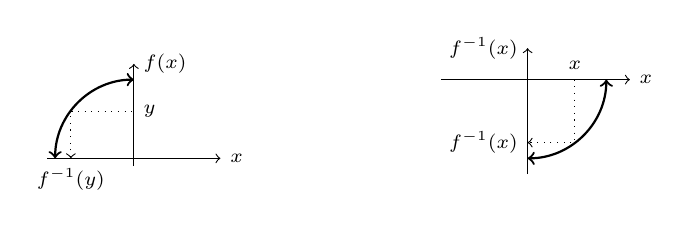
\begin{tikzpicture}
 \draw[ ->] (-1.1,0)--(1.1,0) node[right]{$\scriptstyle{x}$};
 \draw[ ->] (0,-0.1)--(0,1.2) node[right]{$\scriptstyle{f(x)}$};
\draw[thick, <->] (0,1) arc (90:180:1);
\pgfmathsetmacro{\x}{-0.8};
\draw (\x,0) node[below]{$\scriptstyle{f^{-1}(y)}$};
\draw[dotted, <-] (\x,0)--(\x,{sqrt(1-(\x)^2)})--(0,{sqrt(1-(\x)^2)}) node[right]{$\scriptstyle{y}$};

\begin{scope}[xshift=5cm, yshift=1cm]
  \draw[ ->] (-1.1,0)--(1.3,0)node[right]{$\scriptstyle{x}$};
  \draw[ ->] (0,-1.2)--(0,0.4)node[left]{$\scriptstyle{f^{-1}(x)}$};
\draw[thick, <->] (0,-1) arc (270:360:1);
\pgfmathsetmacro{\x}{0.6};
\draw (\x,0) node[above]{$\scriptstyle{x}$};
\draw[dotted, ->] (\x,0)--(\x,{-sqrt(1-(\x)^2)})--(0,{-sqrt(1-(\x)^2)}) node[left]{$\scriptstyle{f^{-1}(x)}$}; 
\end{scope}
 \end{tikzpicture}\end{bmlimage}
\end{center}
\end{sol}
\end{exo}

\begin{exo}
Considere $f:(-1,\infty)\to \bR$, $f(x)=\frac{1}{x+1}$. A partir do gráfico de $f$, dê o
seu conjunto imagem, e mostre que $f:(-1,\infty)\to \imagem(f)$ 
é uma bijeção. Em seguida, dê a sua função inversa.
\begin{sol}
O gráfico de $\frac{1}{x+1}$ é o de $\tfrac1x$ transladado de uma unidade para a esquerda.
O conjunto imagem é $(0,\infty)$. De fato, para todo $y\in (0,\infty)$, a equação $y=\frac{1}{x+1}$
possui uma solução dada por $x=\frac{1-y}{y}$. Logo, $f^{-1}:(0,\infty)\to (-1,\infty)$,
$f^{-1}(x)=\frac{1-x}{x}$.
\end{sol}
\end{exo}

\begin{exo}
Seja $f:\bR\to \bR$ uma bijeção ímpar. Mostre que a sua função inversa
$f^{-1}:\bR\to\bR$ é ímpar também.  
\begin{sol}
Para verificar que $f^{-1}(-y)=-f^{-1}(y)$, usemos a definição: seja $x$ o único
$x$ tal que $f^{-1}(-y)=x$. Pela definição de função inversa ($(f\circ
f^{-1})(y)=y$), aplicando
$f$ temos $-y=f(x)$. Portanto, $y=-f(x)=f(-x)$ (pela imparidade de $f$).
Aplicando agora $f^{-1}$ obtemos $f^{-1}(y)=-x$, isto é, $x=-f^{-1}(y)$. Isso
mostra que
$f^{-1}(-y)=-f^{-1}(y)$.
\end{sol}
\end{exo}

\begin{exo}
%(do Prof. Michel Spira)
%Michel
Para cada um dos contradomínios $C$ a seguir, dê um exemplo explícito de bijeção
$f:(0,1)\to C$.
\begin{multicols}{3}
\begin{enumerate}
 \item\label{itexobijecoes1} $(0,b)$, onde $b>0$.
\item\label{itexobijecoes2} $(a,b)$, onde $a<b$.
\item\label{itexobijecoes3} $(0,\infty)$
\item\label{itexobijecoes4} $(-\infty,\infty)$
\item\label{itexobijecoes5} $(0,1)$
%\item $[0,1]$ (difícil!)
\end{enumerate}
\end{multicols}
\vspace{0.01cm}
\begin{sol}
Exemplos:
\eqref{itexobijecoes1} $f(x)=bx$
\eqref{itexobijecoes2} $f(x)=a+(b-a)x$
\eqref{itexobijecoes3} $f(x)=\tan \pisobredois{x}$, ou $f(x)=\tfrac{1}{(x-1)^2}-1$
\eqref{itexobijecoes4} $f(x)=\tan (\tfrac{2}{\pi}(x-\tfrac12))$
\end{sol}
\end{exo}

\begin{exo}
Sejam $f(x)$ e $g(x)$, $x\in \bR$, definidas por 
$$
f(x)\pardef \lfloor x \rfloor+(x-\lfloor x\rfloor)^2\,,\quad
g(x)\pardef \lfloor x \rfloor+\sqrt{x-\lfloor x\rfloor}\,.
$$
Mostre que $g=f^{-1}$.
\end{exo}

\subsection{Inversos das potências}\label{Sec:InversoPotencias}\index{potência! inverso
de}
Vimos que se $p$ é par, então a função $f(x)=x^p$ é par, e 
$\imagem(f)=[0,\infty)$ ou $(0,\infty)$ (dependendo de $p$ ser $>0$ ou $<0$). 
Logo, para serem invertidas, o domínio delas precisa ser restringido. 
Escolheremos (para $p$ par)
\begin{align*}
 f:[0,\infty)&\to [0,\infty)\\
x&\mapsto x^p\,.
\end{align*}
Vemos que com essa restrição, $f$ se torna 
bijetiva: para cada $y\in [0,\infty)$ existe um único $x\in [0,\infty)$ tal que $x^p=y$.
Esse $x$ costuma ser denotado por $x=y^{1/p}$:
\begin{align*}
 f^{-1}: [0,\infty)&\to[0,\infty)\\
y&\mapsto y^{1/p}\,.
\end{align*}
No caso $p=2$, $y^{1/2}= \sqrt{y}$ é a função \grasA{raiz quadrada}. 
\begin{center}
\begin{bmlimage}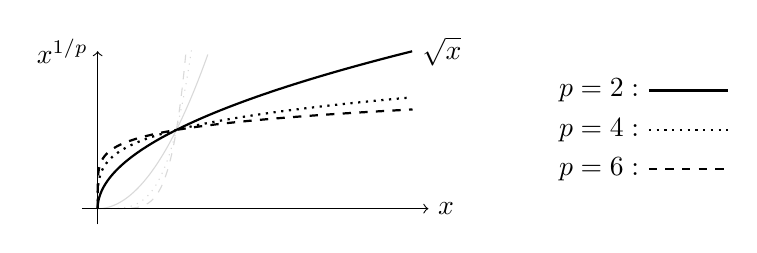
\begin{tikzpicture}[scale=1]
\pgfmathsetmacro{\a}{1.2}
\draw [color=gray!30, dotted, domain=0:\a, samples=100] plot (\x,{\x^4});
\pgfmathsetmacro{\a}{1.12}
\draw [color=gray!30, dashed, domain=0:\a, samples=100] plot (\x,{\x^6});
\pgfmathsetmacro{\a}{1.4}
\draw [color=gray!30, domain=0:\a, samples=100] plot (\x,{(\x)^2});
%\fill (-1,1) circle (0.35mm);
%\fill (1,1) circle (0.35mm);
\pgfmathsetmacro{\a}{1.41}
\draw [thick, dotted, domain=0:\a, samples=100] plot ({\x^4},\x);
\pgfmathsetmacro{\a}{1.26}
\draw [thick, dashed, domain=0:\a, samples=100] plot ({\x^6},\x);
\pgfmathsetmacro{\a}{2}
\draw [thick, domain=0:\a, samples=100] plot ({(\x)^2},\x) node[right]{$\sqrt{x}$};
\draw [ ->] (-0.2,0)--(4.2,0) node[right]{$x$};
\draw [ ->] (0,-0.2)--(0,{2}) node[left]{$x^{1/p}$};
\pgfmathsetmacro{\b}{7};
\pgfmathsetmacro{\c}{1.5};
\draw (\b,\c) node[left]{$p=2:$};
\draw[thick] (\b,\c)--(\b+1,\c);
\draw (\b,\c-0.5) node[left]{$p=4:$};
\draw[thick, dotted] (\b,\c-0.5)--(\b+1,\c-0.5);
\draw (\b,\c-1) node[left]{$p=6:$};
\draw[thick, dashed] (\b,\c-1)--(\b+1,\c-1);
\end{tikzpicture}\end{bmlimage}
\end{center}

Se $p>0$ for ímpar, $\imagem(f)=\bR$ e não é preciso restringir o seu domínio: 
\begin{align*}
 f:\bR &\to \bR\\
x&\mapsto x^p
\end{align*}
é bijetiva, e o seu inverso tem o seguinte gráfico:
\begin{center}
\begin{bmlimage}\begin{tikzpicture}[scale=1]
\pgfmathsetmacro{\a}{1.15}
\draw [color=gray!30, dotted, domain=-\a:\a, samples=100] plot (\x,{\x^3});
\pgfmathsetmacro{\a}{1.1}
\draw [color=gray!30, dashed, domain=-\a:\a, samples=100] plot (\x,{\x^5});
\pgfmathsetmacro{\a}{1.3}
\draw [thick, dotted, domain=-\a:\a, samples=100] plot ({\x^3},\x);
\pgfmathsetmacro{\a}{1.2}
\draw [thick, dashed, domain=-\a:\a, samples=100] plot ({\x^5},\x);
\draw [ ->] (-2.5,0)--(2.5,0) node[right]{$x$};
\draw [ ->] (0,-1.5)--(0,1.5) node[left]{$x^{1/p}$};
\pgfmathsetmacro{\b}{5};
\pgfmathsetmacro{\c}{1.5};
%\draw (\b,\c) node[left]{$p=1:$};
%\draw[thick] (\b,\c)--(\b+1,\c);
\draw (\b,\c-0.5) node[left]{$p=3:$};
\draw[thick, dotted] (\b,\c-0.5)--(\b+1,\c-0.5);
\draw (\b,\c-1) node[left]{$p=5:$};
\draw[thick, dashed] (\b,\c-1)--(\b+1,\c-1);
\end{tikzpicture}\end{bmlimage}
\end{center}


\begin{exo}
Complete essa discussão, incluindo os valores negativos de $p$.
\end{exo}

\begin{exo}
Resolva:
\begin{multicols}{3}
\begin{enumerate}
\item\label{itexoresolvagraf1} $x>\sqrt{x+2}$
\item\label{itexoresolvagraf2} $(x-1)^2\leq \sqrt{1-x}$
\item\label{itexoresolvagraf3} $\sqrt{-x^2-x+6}=-(x+1)$
\end{enumerate}
\vspace{0.04cm}
\end{multicols}
\begin{sol}
\ref{itexoresolvagraf1} $S=(\frac{1+\sqrt{5}}{2},+\infty)$
\ref{itexoresolvagraf2} $S=[0,1]$
\ref{itexoresolvagraf2} $S=\{-\tfrac52\}$
\end{sol}
\end{exo}

\subsection{Funções trigonométricas inversas}\label{Sec:Functriginversas}
Vimos que para a função $\sen: \bR\to [-1,1]$, 
um $y\in [-1,1]$ possui infinitas preimagens, logo não é bijeção. 
Portanto, para \emph{inverter} a função seno, é necessário restringir o seu domínio. A restringiremos ao intervalo  $[-\pisobredois,\pisobredois]$:
\begin{center}
\begin{bmlimage}\begin{tikzpicture}
\draw [->] (-3.5,0)--(3.5,0) node[right]{$x$};
\draw [->] (0,-1.3)--(0,1.3) node[right]{$\sen x$};
%\draw [color=gray!30, domain=-3.5:3.5] plot (\x,{sin(\x r)}); 
\draw [thick, domain=-1.57:1.57, samples=50] plot (\x,{sin(\x r)}); 
\draw (-1.57,0) node[above]{$\scriptstyle{-\pisobredois}$};
\draw (1.57,0) node[below]{$\scriptstyle{\pisobredois}$};
\draw [dashed] (-1.57,0)--(-1.57,-1);
\draw [dashed] (1.57,0)--(1.57,1);
\draw [dashed] (0,1) node[left]{$\scriptstyle{1}$}--(1.57,1);
\draw [dashed] (0,-1) node[right]{$\scriptstyle{-1}$}--(-1.57,-1);
\pgfmathsetmacro{\a}{0.8};
\draw [dotted, <->] (\a,0) node[below]{$\scriptscriptstyle{x}$}--(\a,{sin(\a r)})--(0,{sin(\a r)}) node[left]{$\scriptstyle{y}$};
\fill (1.57,1) circle (0.45mm);
\fill (-1.57,-1) circle (0.45mm);
\end{tikzpicture}\end{bmlimage}
\end{center}
De fato, com essa restrição,
\begin{align*}
\sen :[-\pisobredois,\pisobredois]&\to [-1,1]\\
x&\mapsto \sen x
\end{align*}
é uma bijeção, pois cada $y\in [-1,1]$ é atingido e possui uma única preimagem. A função
inversa é chamada \grasA{arcseno}\index{$\arcsen$}, e denotada
\begin{align*}
\arcsen :[-1,1]&\to [-\pisobredois,\pisobredois]\\
y&\mapsto \arcsen y\,.
\end{align*}
Pela sua definição, ela satisfaz:
\begin{equation}
\boxed{ \forall y\in [-1,1]:\,\sen (\arcsen y)=y\,\,,\quad\text{ e } 
\quad\forall x\in [-\pisobredois,\pisobredois]:\,\arcsen(\sen
x)=x\,\,.}
\end{equation}

 O gráfico de $\arcsen$ pode ser obtido por uma reflexão do gráfico de $\sen$ pela
diagonal do primeiro quadrante:
\begin{center}
\begin{bmlimage}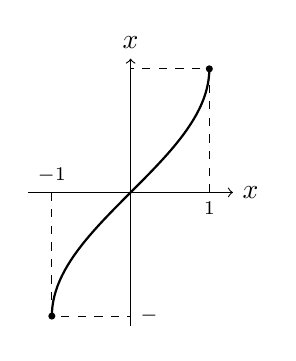
\begin{tikzpicture}
\draw [->] (-1.3,0)--(1.3,0) node[right]{$x$};
\draw [->] (0,-1.7)--(0,1.7) node[above]{$\arcsen x$};
%\draw [color=gray!30, domain=-3.5:3.5] plot ({sin(\x r)},\x); 
\draw [thick, domain=-1.57:1.57, samples=50] plot ({sin(\x r)},\x); 
\draw [dashed] (1,0) node[below]{$\scriptstyle{1}$}--(1,1.57)--(0,1.57) node[left]{$\scriptstyle{\pisobredois}$};
\draw [dashed] (-1,0) node[above]{$\scriptstyle{-1}$}--(-1,-1.57)--(0,-1.57) node[right]{$\scriptstyle{-\pisobredois}$};
\pgfmathsetmacro{\a}{0.8};
% \draw [dotted, <->] (0,\a) node[below]{$\scriptscriptstyle{x}$}--(\a,{sin(\a r)})--(0,{sin(\a r)}) node[left]{$\scriptstyle{y}$};
\fill (1,1.57) circle (0.45mm);
\fill (-1,-1.57) circle (0.45mm);
\end{tikzpicture}\end{bmlimage}
\end{center}
\begin{obs} (Já fizemos esse comentário no Exemplo \ref{exemploinversao}.)
 Como $\arcsen$ é definida como a função inversa de $x\mapsto \sen x$ (no intervalo
$[-\pisobredois, \pisobredois]$), o mais correto é escrevê-la $y\mapsto \arcsen y$.
 Mas para esboçar o seu gráfico, faz mais sentido usar a notação habitual, em que o eixo
das abscissas é chamado de ``$x$''. Por isso, esse último gráfico representa o gráfico da
função $\arcsen$, mas chamando a sua variável $x$ (em vez de $y$): 
$x\mapsto \arcsen x$.
Faremos a mesma modificação nos próximos gráficos.
\end{obs}

\begin{exo}
Seja $y\in (0,\pisobredois)$ tal que $y=\arcsen\tfrac35$. Calcule $\sen y$, $\cos y$, e
$\tan y$.
\begin{sol}
Por definição, $\sen y=\tfrac35$. Logo, $\cos y=+\sqrt{1-\sen^2 y}=\tfrac45$ (a raiz
positiva é escolhida, já que $y\in (0,\pisobredois)$). Portanto, $\tan y=\tfrac34$.
\end{sol}
\end{exo}

O cosseno pode ser invertido também, uma vez que o seu domínio é bem escolhido:
\begin{align*}
\cos :[0,\pi]&\to [-1,1]\\
x&\mapsto \cos x
\end{align*}
\begin{center}
\begin{bmlimage}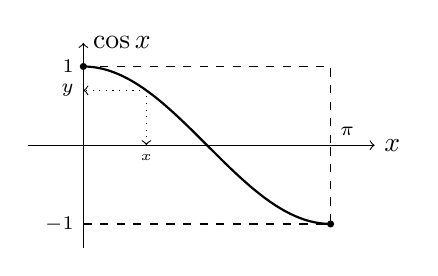
\begin{tikzpicture}
\draw [->] (-0.7,0)--(3.7,0) node[right]{$x$};
\draw [->] (0,-1.3)--(0,1.3) node[right]{$\cos x$};
%\draw [color=gray!30, domain=-1:3.7] plot (\x,{cos(\x r)}); 
\draw [thick, domain=0:3.14, samples=50] plot (\x,{cos(\x r)}); 
%\draw (-1.57,0) node[above]{$\scriptstyle{-\pisobredois}$};
\draw (3.14,0) node[above right]{$\scriptstyle{\pi}$};
\draw [dashed] (0,1) node[left]{$\scriptstyle{1}$}--(3.14,1)--(3.14,0);
\draw [dashed] (0,-1) node[left]{$\scriptstyle{-1}$}--(3.14,-1)--(3.14,0);
\pgfmathsetmacro{\a}{0.8};
 \draw [dotted, <->] (\a,0) node[below]{$\scriptscriptstyle{x}$}--(\a,{cos(\a
r)})--(0,{cos(\a r)}) node[left]{$\scriptstyle{y}$};
\fill (0,1) circle (0.45mm);
\fill (3.14,-1) circle (0.45mm);
\end{tikzpicture}\end{bmlimage}
\end{center}
A função inversa é chamada \grasA{arcosseno}\index{$\arcos$}, e denotada
\begin{align*}
\arcos :[-1,1]&\to [0,\pi]\\
y&\mapsto \arcos y\,.
\end{align*}
Ela possui as propriedades:
\begin{equation}\label{eq:identarseno1}
\boxed{ \forall y\in [-1,1]:\,\cos (\arcos y)=y\,\,,\quad\text{ e } 
\quad\forall x\in [0,\pi]:\,\arcos(\cos x)=x\,\,.}
\end{equation}

O gráfico de $\arcos$ pode ser obtido por uma reflexão pela diagonal do primeiro quadrante:

\begin{center}
\begin{bmlimage}\begin{tikzpicture}
\draw [->] (-1.3,0)--(1.3,0) node[right]{$x$};
\draw [->] (0,-0.3)--(0,3.5) node[above]{$\arcos x$};
%\draw [color=gray!30, domain=-3.5:3.5] plot ({sin(\x r)},\x); 
\draw [thick, domain=0:3.14, samples=50] plot ({cos(\x r)},\x); 
 \draw  (1,0) node[below]{$\scriptstyle{1}$};
\draw [dashed] (-1,0) node[below]{$\scriptstyle{-1}$}--(-1,3.14)--(0,3.14) node[right]{$\scriptstyle{\pi}$};
\pgfmathsetmacro{\a}{0.8};
\fill (1,0) circle (0.45mm);
\fill (-1,3.14) circle (0.45mm);
\end{tikzpicture}\end{bmlimage}
\end{center}


Para inverter a tangente, faremos a restrição 
\begin{align*}
 \tan :(-\pisobredois,\pisobredois)&\to \bR\\
x&\mapsto \tan x\,,
\end{align*}
obtendo assim uma bijeção.
\begin{center}
\begin{bmlimage}\begin{tikzpicture}
\pgfmathsetmacro{\eps}{0.3};
\pgfmathsetmacro{\pisd}{1.5707};
\pgfmathsetmacro{\h}{3};
\begin{scope}
%\draw[color=gray!70, dashed] (-3*\pisd,-\h)--(-3*\pisd,+\h);
%\draw [color=gray!70, domain={-3*\pisd+\eps}:{-\pisd-\eps}, samples=100] plot
%(\x,{(sin(\x r))/(cos(\x r))});
\draw[dashed] (-\pisd,-\h)--(-\pisd,+\h);
\draw [thick, domain={-\pisd+\eps}:{\pisd-\eps}, samples=100] plot (\x,{(sin(\x r))/(cos(\x r))});
\draw[dashed] (\pisd,-\h)--(\pisd,+\h);
%\draw [color=gray!70, domain={\pisd+\eps}:{3*\pisd-\eps}, samples=100] plot (\x,{(sin(\x
%r))/(cos(\x r))});
%\draw[color=gray!70, dashed] (3*\pisd,-\h)--(3*\pisd,+\h);
\draw [ ->] (-6,0)--(6,0) node[right]{$x$};
\draw [ ->] (0,-2.3)--(0,{2.3}) node[above]{$\tan x$};
\draw[dotted, <->] (1,0) node[below]{$x$}--(1,{tan(1 r)})--(0,{tan (1 r)}) node[left]{$y$};
\fill (1,{tan(1 r)}) circle (0.28mm);
\end{scope}
\end{tikzpicture}\end{bmlimage}
\end{center}
A função inversa é chamada de \grasA{arctangente}\index{$\arctan$}:
\begin{align*}
 \arctan :\bR&\to (-\pisobredois,\pisobredois)\\
y&\mapsto \arctan y\,.
\end{align*}
Como antes,
\begin{equation}
\boxed{\forall x\in (-\pisobredois,\pisobredois):\,\arctan (\tan 
x)=x\,\,,\quad\text{ e }\quad \forall
y\in \bR:\,\tan(\arctan y)=y\,\,.}
\end{equation}
 O seu gráfico possui duas \emph{assíntotas horizontais}: quando $x$ é 
positivo e grande, o gráfico de $\arctan x$ se aproxima da reta de equação 
$y=\pisobredois$, e quando $x$ é
negativo e grande, ele  se aproxima da reta de equação $y=-\pisobredois$:
\begin{center}
\begin{bmlimage}\begin{tikzpicture}
\pgfmathsetmacro{\eps}{0.2};
\pgfmathsetmacro{\pisd}{1.5707};
\pgfmathsetmacro{\h}{5};
\begin{scope}
\draw[dashed] (-\h,-\pisd)--(\h,-\pisd);
 \draw [thick, domain={-\pisd+\eps}:{\pisd-\eps}, samples=100] plot ({(sin(\x r))/(cos(\x
r))},\x);
\draw[dashed] (-\h,\pisd)--(\h,\pisd);
\draw [->] (-\h,0)--(\h,0) node[right]{$x$};
\draw [ ->] (0,-2)--(0,2) node[right]{$\arctan x$};
%\draw[dotted, <->] (0,1) node[below]{$x$}--({tan(1 r)},1)--({tan (1 r)},0) node[left]{$y$};
\end{scope}
\end{tikzpicture}\end{bmlimage}
\end{center}
Observemos também que $\arctan$ é uma função ímpar, limitada por $\pisobredois$. 

\begin{obs}
 É importante notar que as três funções trigonométricas inversas, $\arcsen$ $\arcos$ e
$\arctan$, foram definidas a partir de uma \emph{escolha} de uma restrição para cada uma
das funções $\sen$, $\cos$ e $\tan$.
Essa escolha pode parecer arbitrária, mas é a mais comum usada nos livros de matemática.
Continuaremos usando as funções inversas assim definidas, até o fim do curso. 
\end{obs}

\begin{exo}
Determine os domínios das seguintes funções.
\begin{multicols}{2}
\begin{enumerate}
\item\label{itdomintriginv1} $\arcos x -\arcsen x$
\item\label{itdomintriginv2} $\arcos (2x)$
\item\label{itdomintriginv3} $\tan (\arcsen x)$
\item\label{itdomintriginv4} $\arcos(\tfrac{2-x^2}{1+x^2})$
\end{enumerate}
\end{multicols}
\vspace{0.1mm}
\begin{sol}
\eqref{itdomintriginv1} $[-1,1]$,
\eqref{itdomintriginv2} $[-\tfrac12,\tfrac12]$,
\eqref{itdomintriginv3} $(-1,1)$,
\eqref{itdomintriginv4} $(-\infty,-\tfrac{1}{\sqrt{2}}]\cup
[\tfrac{1}{\sqrt{2}},+\infty)$.
\end{sol}
\end{exo}

\begin{exo}\label{Exo:Telao}
Uma tela de cinema de $5$ metros de altura está pregada numa parede, $3$ metros acima do chão.
a) Se $P$ é um ponto no chão a distância $x$ da parede, calcule o ângulo $\theta$ sob o qual 
$P$ vê a tela, em função de $x$. 
b) Mesma coisa se $P$ é a $2$ metros do chão.
(Obs: no Exercício \ref{Exo:TelaoBIS} calcularemos onde colocar o ponto $P$ de modo tal que o ângulo 
seja máximo.)
\begin{sol}
Seja $A$ a posição do topo da tela, $B$ a sua base, e $Q$ o ponto onde a parede toca o chão.
Seja $\alpha$ o ângulo $APQ$ e $\beta$ o ângulo $BPQ$.
Temos $\tan \alpha=\tfrac8x$, $\tan \beta=\tfrac3x$. Logo, em a): 
$\theta(x)=\arctan\tfrac8x-\arctan\tfrac3x$. Em
b), $\theta(x)=\arctan\tfrac6x-\arctan\tfrac1x$. 
\end{sol}
\end{exo}

\begin{exo}
Resolva:
\begin{multicols}{3}
\begin{enumerate}
\item\label{itexoinvtrig1} $3\arcsen x=\pisobredois$
\item\label{itexoinvtrig2} $\arctan (x-1)=\tfrac{\pi}{3}$
\item\label{itexoinvtrig3} $2\sen (\arcsen x)=\tfrac13$
\item\label{itexoinvtrig4} $\arctan(\tan (x^2))=\tfrac{\pi}{9}$
\end{enumerate}
\end{multicols}
\vspace{0.01cm}
\begin{sol}
\eqref{itexoinvtrig1} $x=\frac{1}{2}$
\eqref{itexoinvtrig2} $x=\sqrt{3}+1$
\eqref{itexoinvtrig3} $x=\tfrac16$
\eqref{itexoinvtrig4} $x=\tfrac{\sqrt{\pi}}{3}$
\end{sol}
\end{exo}

As funções trigonométricas inversas têm identidades associadas. Somente consideraremos algumas:
\begin{ex}\label{Ex:identidadesenoinverso}
Provemos, por exemplo, a identidade
\eq{\cos(\arcsen x)=\sqrt{1-x^2}\,,\quad\forall x\in [-1,1]\,.}
Primeiro, como
$\sen^2\alpha+\cos^2\alpha=1$, temos, usando \eqref{eq:identarseno1}, 
$$\cos^2(\arcsen
x)=1-\sen^2(\arcsen x)=1-x^2\,.$$
Mas como $-\pisobredois\leq \arcsen x\leq \pisobredois$, vale 
$\cos(\arcsen x)\in [0,1]$, logo, tomando a raiz quadrada dá a 
idendidade desejada.
Um outro jeito de entender a identidade é de escrevê-la como 
$\cos(\arcsen x)=\cos \alpha$, onde 
 $\alpha=\arcsen x$. Logo, $\sen \alpha=x$, o que pode ser representado 
num triângulo:

\begin{center}
\begin{bmlimage}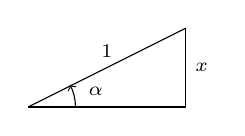
\begin{tikzpicture}[scale=2]
\draw (0,0)--(1,0)--(1,0.5) node[midway, right]{$\scriptstyle{x}$};
\draw (1,0.5)--(0,0) node[midway, above]{$\scriptstyle{1}$};
\draw[ ->] (0.3,0) arc (0:28:0.3);
\draw (0.43,0.1) node{$\scriptstyle{\alpha}$};
\end{tikzpicture}\end{bmlimage}
\end{center}
Nesse triângulo vemos que $\cos \alpha=\tfrac{\sqrt{1-x^2}}{1}=\sqrt{1-x^2}$.
\end{ex}

\begin{exo} Simplifique:
\begin{multicols}{3}
 \begin{enumerate}
\item\label{itidenttriginv1} $\cos(2\arcos x)$
\item\label{itidenttriginv2} $\cos(2\arcsin x)$
\item\label{itidenttriginv3} $\sen(2\arcos x)$
\item\label{itidenttriginv4} $\cos(2\arctan x)$
\item\label{itidenttriginv5} $\sen (2\arctan x)$
\item\label{itidenttriginv6} $\tan (2\arcsen x)$
 \end{enumerate}
\end{multicols}
\vspace{0.01cm}
\begin{sol}
\eqref{itidenttriginv1} $\cos(2\arcos x)=2\cos^2(\arcos x)-1=2x^2-1$
\eqref{itidenttriginv2} $\cos(2\arcsin x)=1-2\sen^2(\arcsen x)=1-2x^2$
\eqref{itidenttriginv3} $\sen(2\arcos x)=2\sen (\arcos x)\cos (\arcos x)=2x\sqrt{1-x^2}$
\eqref{itidenttriginv4} $\cos(2\arctan x)=2\cos^2(\arctan x)-1=\tfrac{1-x^2}{1+x^2}$
\eqref{itidenttriginv5} $\sen (2\arctan x)=\frac{2x}{1+x^2}$
\eqref{itidenttriginv6} $\tan (2\arcsen x)=\frac{2x\sqrt{1-x^2}}{1-2x^2}$
\end{sol}
\end{exo}

\begin{exo}
Mostre que para todo $x\in [-1,1]$, 
$$
\arcsen x+\arcos x=\tfrac{\pi}{2}\,.
$$
\begin{sol}
Chamando $\alpha=\arcsen x$, $\beta=\arcos x$, temos $x=\sen \alpha$, $x=\cos \beta$:
\begin{center}
\begin{bmlimage}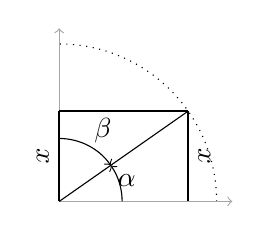
\begin{tikzpicture}[scale=2]
\pgfmathsetmacro{\a}{1};
\draw[dotted] (\a,0) arc (0:90:\a);
\draw[ ->, color=gray!70] (0,0) -- (1.1*\a,0);
\draw[ ->, color=gray!70] (0,0) -- (0,1.1*\a);
\pgfmathsetmacro{\alf}{35};
\coordinate (P) at ({0.4*\a*cos(\alf)},{0.4*\a*sin(\alf)});
\draw[<-] (P) arc (\alf:90:{0.4*\a});
\draw[->] ({0.4*\a},0) arc (0:\alf:{0.4*\a});
\draw ({\alf/2}:{0.45*\a}) node{$\alpha$};
\draw ({\alf+(90-\alf)/2}:{0.35*\a}) node[above right]{$\beta$};
\coordinate (B) at ({\a*cos(\alf)},{\a*sin(\alf)});
\coordinate (Bx) at ({\a*cos(\alf)},0);
\coordinate (By) at (0,{\a*sin(\alf)});
\draw (0,0)--(B);
\draw [thick] (B)--(Bx) node[midway, above, sloped]{$x$};
\draw [thick] (By)--(B);
\draw [thick] (By)--(0,0) node[midway, below, sloped]{$x$};
\end{tikzpicture}\end{bmlimage}
\end{center}
\end{sol}
\end{exo}

%VER EXOS DOUCHET p.54







